\chapter{Analysis}
\label{chap:analysis}

In this chapter we analyse the performance of the RP method for online outlier detection in multivariate time series. We explain the analysis setup in section \ref{sec:analysis_methodology}, after which we provide more insight in the inner working of the RP method in section \ref{sec:analysis_innerworking}. In section \ref{sec:analysis_bird} we analyse the method under varying parameter settings. We also investigate the influence of back-scaling for different types of outliers. In section \ref{sec:analysis_contextual} we explain how we use the method in a slightly different manner, and analyse its performance accordingly. Section \ref{sec:analysis_worm} presents the performances under fixed parameter settings to assess both uses of the method in online mode. Section \ref{sec:analysis_concluding} concludes with a summary of the key findings.


\section{Analysis setup}
\label{sec:analysis_methodology}

In this thesis, we focus on the task of online unsupervised outlier detection in multivariate time series. We discussed the most important challenges imposed by this task in table \ref{tab:intro_characteristics}. The central objective of this analysis is to assess the applicability of the proposed method given these challenges. To that end, we translated them into a set of evaluation criteria which we, in turn, linked to measurable performance metrics to guide this analysis and the real-world experiments following in chapter \ref{chap:experiments}. This translation is presented in table \ref{tab:analysis_evaluation}. 

In the remainder of this section we explain the synthetic data and performance metrics used for the analysis. Obviously, a method can be optimized such that it evaluates very well given one criterion, but performs horrible given another. Therefore, we make up a qualitative comparative judgement on the criteria all together in section \ref{sec:analysis_concluding}.

\begin{table}[h]
	\centering
	\hspace{-0.5cm}
	\vspace{-0.25cm}
	\caption{Evaluation criteria for this analysis and the real-world experiments in chapter \ref{chap:experiments}.}
	\label{tab:analysis_evaluation}
	\small
	\begin{tabular}{l l l}
		\toprule
		\textbf{Challenge} & \textbf{Evaluation criterion} & \textbf{Performance metric}\\ \midrule
		The algorithm must assign label $O_i$ 		& 	\multirow{2}{*}{Time needed to process data points} &  \multirow{2}{*}{Runtime performance.}	\\
		to data point $\mathbf{x}_i$ before receiving $\mathbf{x}_{i+1}$	& 	&		 \\[0.15cm]
		The algorithm should only need a limited	& \multirow{2}{*}{Dependence on history of stream} & Number of preceding  \\
		history of the data to infer its model & & data points $p$ needed. \\[0.15cm]
		
		The algorithm should run unsupervised & Amount of prior information needed & Number of parameters.\\[0.15cm]
		The detection performance should not be & Sensitivity of detection	performance to & \multirow{2}{*}{Detection performance.} \\
		too sensitive to the (fixed) parameters & parameters &  \\ \midrule
		
		The analyst should have an idea 	& Generalizability of performances to  & Stability of detection and \\
		of the data and outliers at hand 	& (un)standardized and different data sets & runtime performance. \\[0.15cm]
		The algorithm should be able to detect & Generalizability of performances to	& Stability of detection  \\
		global and contextual outliers & different outlier types 			& performance. \\ \midrule
		
		The algorithm should be able to find 	& Influence of $d$ and $n$ on detection		& Scalability of detection \\
		outliers in high-dimensional data 		& performance 			& performance. \\[0.15cm]
		Algorithms should scale in computational &	\multirow{2}{*}{Influence of $d$ on	runtime performance} & Scalability of runtime \\
		complexity with increasing $d$ 	& 		& performance.\\ \bottomrule		
	\end{tabular}
\vspace{-0.3cm}
\end{table}

\subsection{Data}

As limited qualitative labelled data sets are available that fully meet the conditions of the considered problem context, we turned to artificial data sets for the in-depth analysis of our method. An assessment of the RP method on real-world data follows in chapter \ref{chap:experiments}.
We kept the structure in our data simple by generating just $60$ time series of length $981$ from sinusoidal functions each with a different phase (sine or cosine), additional random misalignment ($\varphi$), amplitude ($A$) and offset ($C$). We also added a time-depending noise term $N_t$ to avoid smooth time series. The specific function underlying each time series in our artificial data set is as follows

\begin{equation}\label{eq:analysis_data}
 \mathbf{x}(t) = 
	\begin{cases} 
		A \sin(t + \varphi) + C + N_t	& \text{with probability } \frac{1}{2} \\[0.5em]
		A \cos(t + \varphi) + C + N_t   & \text{with probability } \frac{1}{2},
	\end{cases}
\end{equation}
\vspace{0.2cm}

\noindent with $t$ from $1$ to $50$ with an interval of $0.05$, $A \sim \mathcal{U}(1,3)$, $\varphi \sim \mathcal{N}(0,1)$, $C \sim \mathcal{U}(0,1)$ and $N_t \sim \mathcal{N}(0,0.05)$. From this point onwards, we refer to each time step $t$ with integer values $i$ from $1$ to $981$. Like in many real-world applications, the distinct time series have a different range and not necessarily $0$ mean. Online procedures are available to standardize the time series to $0$ mean with unit variance, of which a common method is discussed in section \ref{sec:analysis_contextual}. In practice such online methods do not perfectly standardize the data over the entire stream. Therefore, to analyse the random projection method in a realistic setting we introduced the offset term $C$. The analysis results with standardized data are presented and discussed in the appendix \ref{app:analysis}.

We created $3$ distinct copies of the resulting $60 \times 981$ clean data set and injected each data set with either global point outliers, contextual point outliers or contextual collective outliers. First, we randomly sampled $6$ distinct subsets of $12$ (out of $60$) time series, where we injected $1$ of the $3$ outlier types in each pair of $2$ subsets. The global point outliers were created by multiplying $6$ random sequences of $3$ data points with an arbitrary large factor of $1.5$, i.e. \{$\tilde{\mathbf{x}}_{i,j} = 1.5 \ \mathbf{x}_{i,j} : i=1,2,3$\} with $j$ the time series from the respective subset. The contextual point outliers were obtained by multiplying $6$ random sequences of $3$ data points with a small enough factor of $0.1$, i.e. \{$\tilde{\mathbf{x}}_{i,j} = 0.1 \ \mathbf{x}_{i,j} : i=1,2,3$\}. The collective outliers were obtained by replacing $4$ random sequences of $15$ data points with the values at the first time step of that time series $j$, i.e. \{$\tilde{\mathbf{x}}_{i,j} = \mathbf{x}_{1,j} : i=1,2,...,15 $\}. The outlier characteristics are summarized in table \ref{tab:analysis_outliers}.

\begin{table}[h]
	\centering
	\caption{Summary of the outliers in the synthetic time series.}
	\label{tab:analysis_outliers}
	\begin{tabular}{l c c c  }
		\toprule	
		\multirow{2}{*}{\textbf{Outlier type}} & \textbf{$\#$ responsive} & \textbf{$\#$ outlying} & \textbf{Feature value} \\
		&  \textbf{time series} & \textbf{data points} & \textbf{of time series $j$} \\
		\midrule
		Global point			& $2$ subsets of $12$	& $6 \cdot 3 = 18$  & $\tilde{\mathbf{x}}_{i,j} = 1.5 \  \mathbf{x}_{i,j}$ 	\\
		Contextual point		& $2$ subsets of $12$ 	& $6 \cdot 3 = 18$  & $\tilde{\mathbf{x}}_{i,j} = 0.1 \  \mathbf{x}_{i,j}$	\\
		Contextual collective	& $2$ subsets of $12$	& $4 \cdot 15 = 45$  & $\tilde{\mathbf{x}}_{i,j} = \mathbf{x}_{1,j}$	\\
		\bottomrule
	\end{tabular}
\end{table}

Parts of $3$ of the $60$ resulting time series with the different outlier types are shown in figures \ref{fig:analysis_point} to \ref{fig:analysis_collective}. Clearly, we have correlating and stationary time series what might be different in real-world applications. In chapter \ref{chap:experiments} we assess and compare the performances on (more) realistic data.

\begin{figure}[h]
	\begin{minipage}{0.333\textwidth}
		\centering
		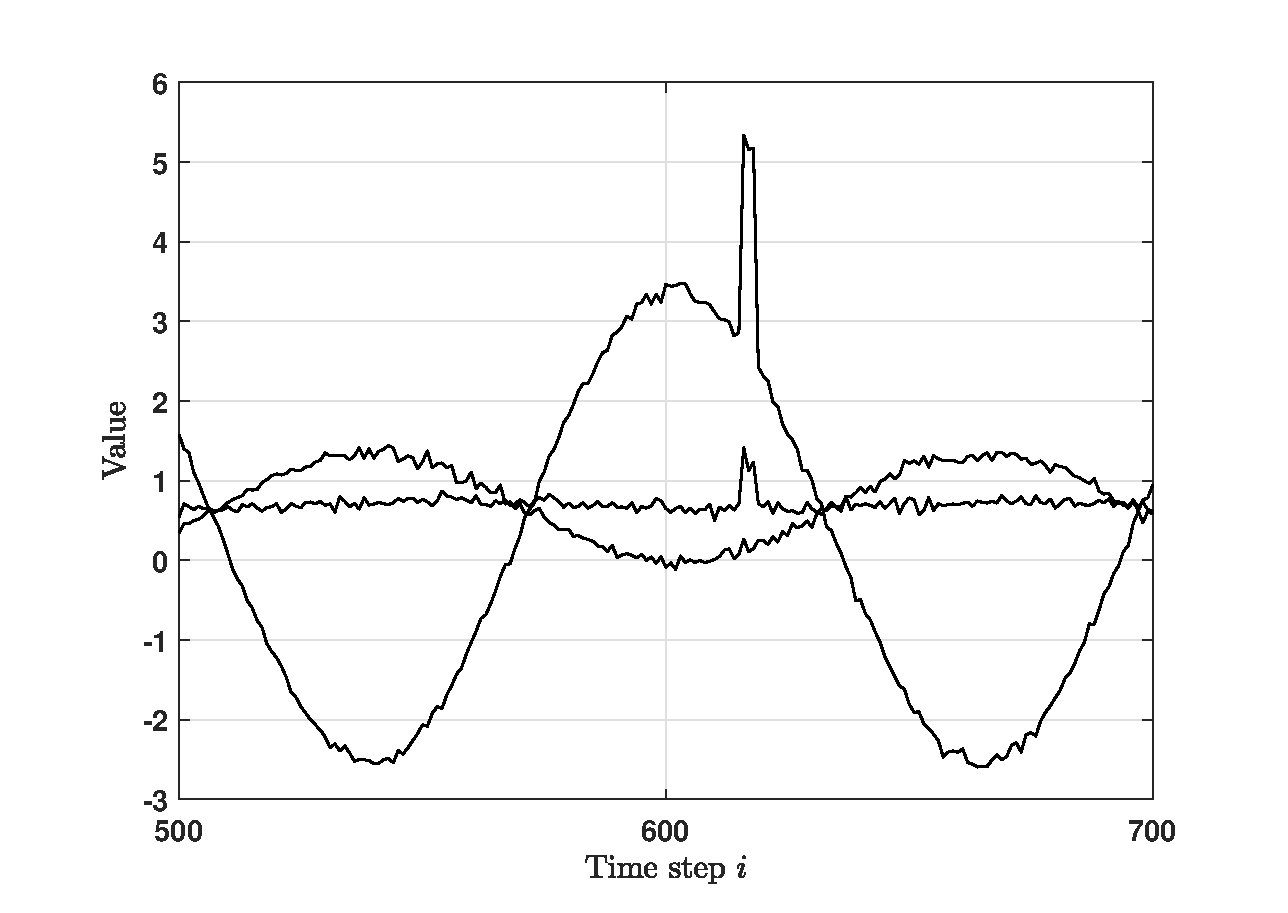
\includegraphics[scale=0.27]{analysis/Example_timeseries_point_frac}
		\caption{Global point}
		\label{fig:analysis_point}
	\end{minipage}
	\begin{minipage}{0.333\textwidth}
		\centering
		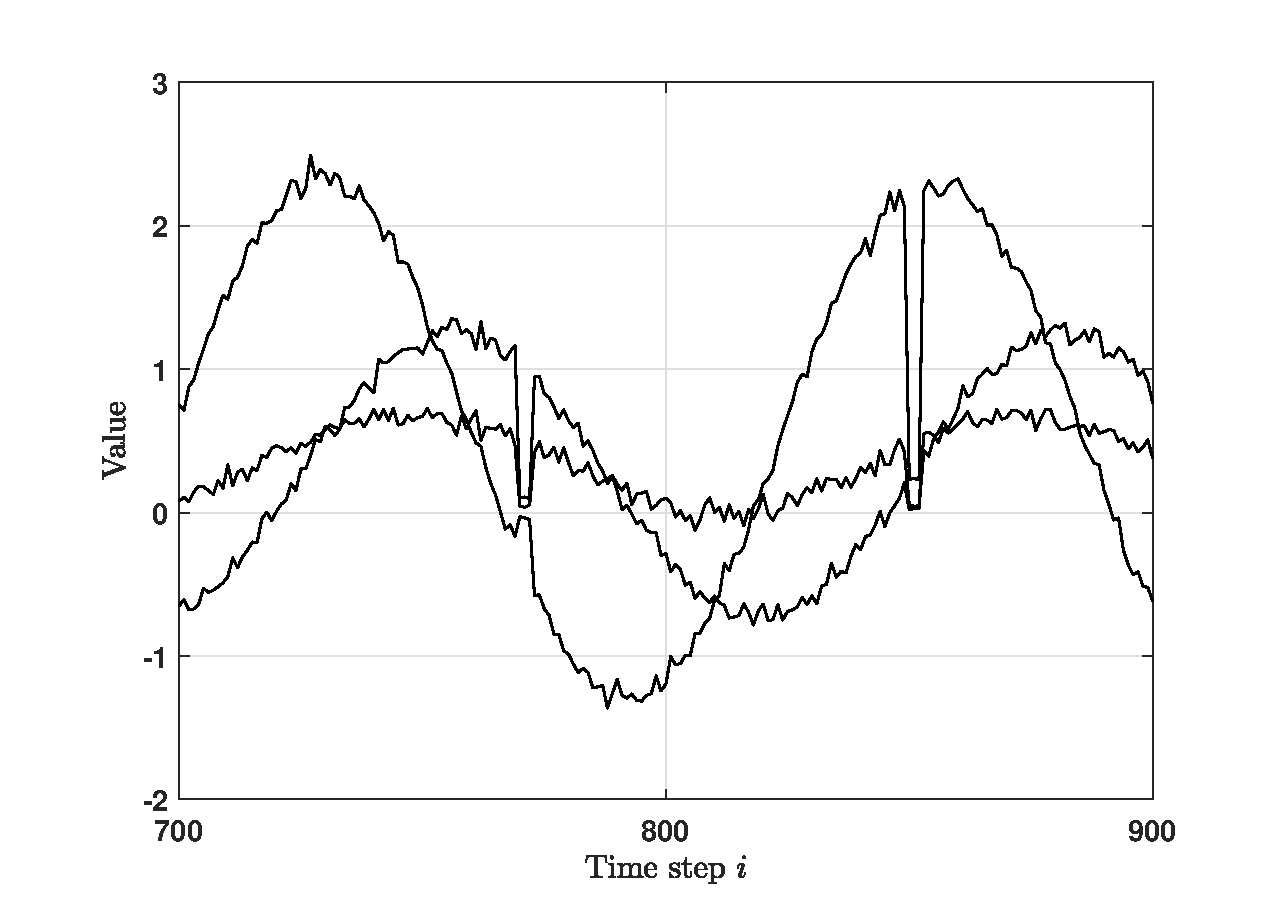
\includegraphics[scale=0.27]{analysis/Example_timeseries_contextual_frac}
		\caption{Contextual point}
		\label{fig:analysis_contextual}
	\end{minipage}
	\begin{minipage}{0.333\textwidth}
		\centering
		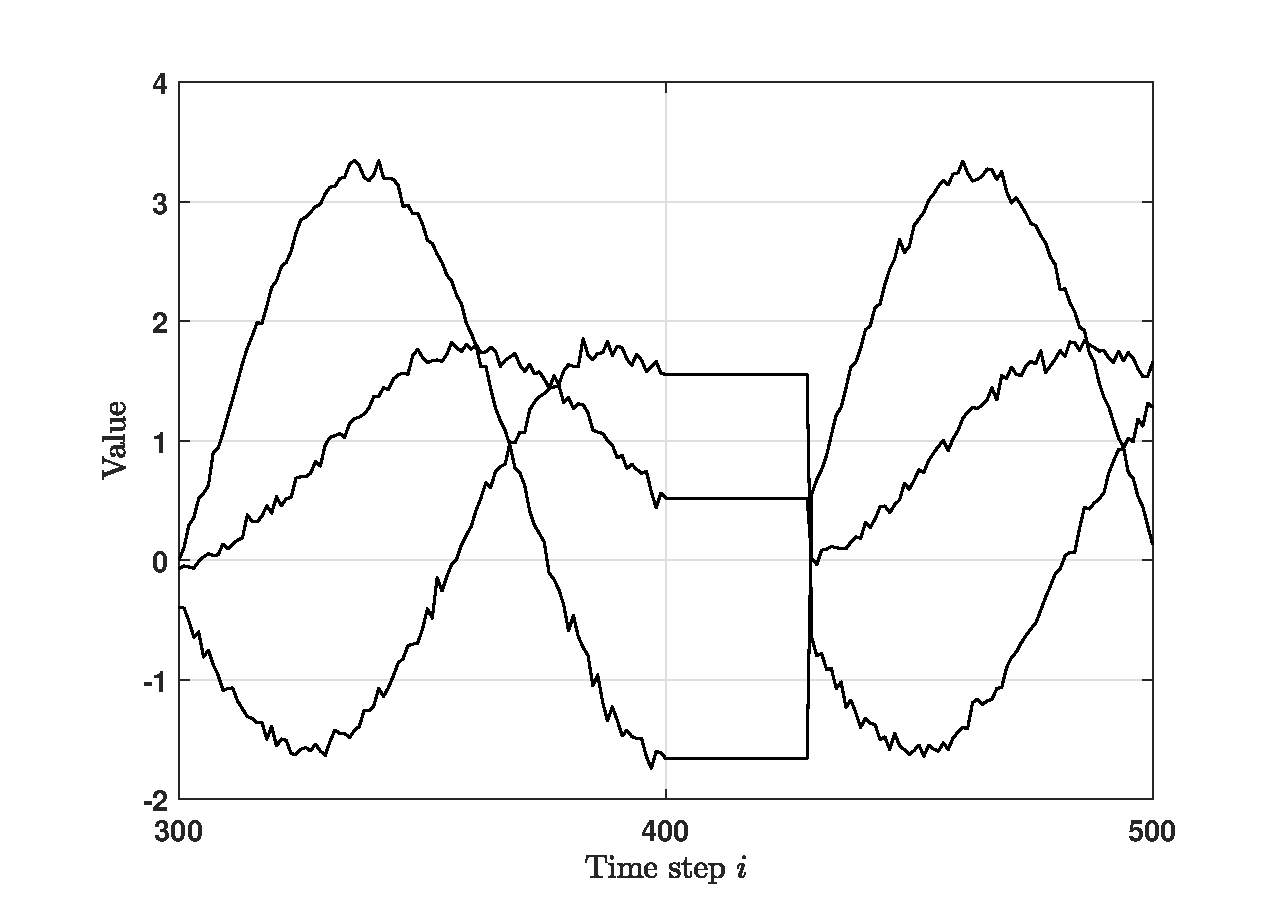
\includegraphics[scale=0.27]{analysis/Example_timeseries_collective_frac}
		\caption{Contextual collective}
		\label{fig:analysis_collective}
	\end{minipage}
\end{figure}

For outlier detection in multivariate time series a sliding window is often implemented to not only look at a single data point $\mathbf{x}_i$ to derive its outlier score, but look at $\mathbf{x}_i$ given its history of length $p$. This way we might be better in detecting interruptions of the temporal continuity exhibited in stream $\mathbf{X}$. Applying a sliding window, therefore, particularly benefits commonly used methods to detect contextual outliers. A sliding window can be established by just concatenating each $\mathbf{x}_i \in \mathbb{R}^d$ with its $p$ previous values $\mathbf{x}_{i-1},\mathbf{x}_{i-2},...,\mathbf{x}_{i-p}$ resulting in $\mathbf{x}_i \in \mathbb{R}^{d \cdot p}$.
Technically this translates to classifying sequences of $p$ data points instead of single data points, but as the window slides only 1 step further we can interpret this as classifying $\mathbf{x}_i$ given its previous $p$ values. Each window $\mathbf{x}_i \in \mathbb{R}^{d \cdot p}$ is labelled as outlier if at least one of the data points $\mathbf{x}_i,...\mathbf{x}_{i-p} \in \mathbb{R}^d$ is an outlier. We end up with $(n − p + 1)$ data points in each data set. 

For this analysis we considered window lengths of $1, 5, 10$ and $15$, where $p=1$ reflects the original data set where no sliding window is implemented and we classify the single data points. In short, we obtained data sets of sizes as in table \ref{tab:analysis_datasets}.

\begin{table}[h]
	\centering
	\caption{Dimensionality of data sets with sliding windows.}
	\label{tab:analysis_datasets}
	\begin{tabular}{ c c c }
		\toprule	
		\textbf{Original} & \multirow{2}{*}{\textbf{Window length $p$}}  & \textbf{Resulting} \\
		\textbf{dimensionality} & & \textbf{dimensionality} \\
		\midrule
		\multirow{4}{*}{$60 \times 981$} & $1$ 	& $60 \times 981 $ 	\\
									 	 & $5$ 	& $300 \times 977$	\\
										 & $10$	& $600 \times 972$ 	\\
										 & $15$	& $900 \times 967$ 	\\
		\bottomrule
	\end{tabular}
\end{table}


\subsection{Performance metrics}

\subsubsection{\textit{Runtime performance}}

Even though we already provided the upper bounds for the runtime complexity of the methods we also investigated their runtime in practice. This enables us to investigate the runtime behaviour of the algorithms for different settings of the parameters. We do not interpret the actual time that it takes to run the algorithms as that depends on machine configurations and is not in our interest, we merely use it as a mean to see how methods compare to each other. For all experiments we measured the time it takes before a method has computed the outlier scores for all $\mathbf{x}_i \in \mathbf{X}$. We used built-in functions $\texttt{tic}$ and $\texttt{toc}$ of Matlab which measure the wall-clock runtime time, i.e. the actual time it takes to execute all operations between commands $\texttt{tic}$ and $\texttt{toc}$. 

\subsubsection{\textit{Number of parameters and preceding data points needed}}
The amount of prior information incorporated in a method is preferred to be minimal in order to make it generalize well to an unseen (and dynamically changing) data stream. The more parameters a method has, the more prior information is needed or guesses have to be made by the analyst to set them properly. Hence, the number of parameters needed to deploy a method seemed to be a good indicator of the prior information consumed by it. 
Altogether, this could make a method suffer from poor generalizability. The number of parameters might however be a bit more nuanced than just being a number. If the analyst has a good idea about a suitable parameter setting before running the system, the number of parameters might not be as critical after all. The impact of this performance metric also strongly coheres with the sensitivity of the detection performance to the parameters.

The number of historic data points needed to process the current data point, if needed at all, by an online method is also considered an important metric. Beside the possible effect on the runtime, it also requires memory storage which is intended to be minimized. As already explained, we created data sets to imitate a sliding window in a data stream. The length $p$ of such a sliding window directly reflects the number of historic data points used. Methods that need a large value for $p$ are less in favour than methods that only need little or no history of a data stream.

\subsubsection{\textit{Detection performance}}

To assess outlier detection methods it is important to realize we are dealing with imbalanced classes. That is, the class of outliers is often much smaller than the class of normal data points. In class-imbalanced situations just taking the ratio of correctly classified data points out of the entire stream does not reflect the detection performance of the method if we want to detect outliers. For example, if we have a classification problem with $95$ normal data points and $5$ outliers, classifying all outliers as normal data points already results in an accuracy of $95\%$. But in that case, we ignore all the outliers we actually wanted to detect with the outlier detection method. 

Instead of simply counting each misclassified data point regardless of whether it is an outlier or normal data point, we separate these counts and refer to outliers as `positives' and the normal data points as `negatives'. Then, a correctly classified outlier is a true positive (TP) and a normal data point classified as an outlier a false positive (FP). Correctly classified normal data points are referred to as true negatives (TN) and outliers classified as being normal as false negatives (FN). 
Eventually we want to find a balance between the number of TP's, FP's, TN's and FN's. For outlier detection methods important metrics that reflect this balance are the True Positive Rate (TPR) and False Positive Rate (FPR) as in equation \eqref{eq:analysis_tprfpr}.

\begin{equation}\label{eq:analysis_tprfpr}
	\text{TPR} = \frac{\text{TP}}{\text{P}} \ , \quad \text{FPR} = \frac{\text{FP}}{\text{N}}
\end{equation}

The TPR reflects the fraction of true detections, i.e. the correctly labelled outliers, over the full number of outliers present in the data. The FPR reflects the fraction of false detections, i.e. the incorrectly labelled normal data points, over the full number of normal data points in the data. The trade-off between these two metrics is found interesting for outlier detection \cite{zimek2012survey}. As we do not implement a threshold method, our method does not output a final label $0$ for normal data points and $1$ for outliers. To that end, we use the Receiver Operating Characteristic (ROC) to inspect the possible balances between the TPR and FPR. The ROC curve computes this balance for all possible thresholds given the outlier scores assigned to the data points. An example of an ROC curve is given in figure \ref{analysis:roc_example}. Each point on this curve represents a possible balance between the TPR and FPR associated with a fixed value for the threshold $\theta$.

\begin{figure}[h]
	\centering
	\vspace{-0.15cm}
	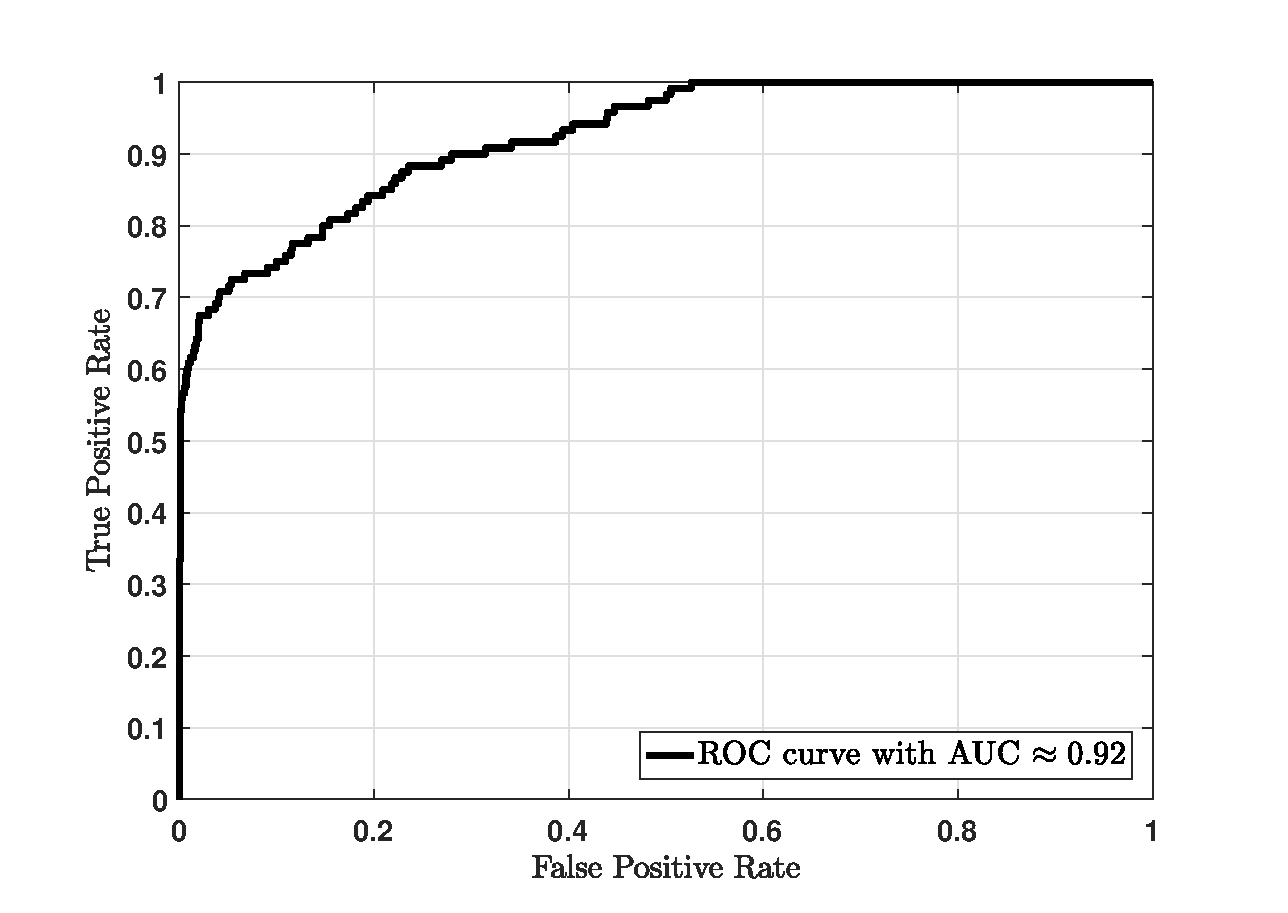
\includegraphics[scale=0.38]{analysis/Example_ROC}
	\caption{Example Receiver Operating Characteristic (ROC) curve.}
	\label{analysis:roc_example}
\end{figure}

Ideally we would have a TPR of $1$ against an FPR of $0$, so we favour methods that result in curves that are closest to the upper left corner. However, for different applications, a different balance between these two criteria is desired. As we do not focus on a particular application and so we do not have a specific desire for this balance, we prefer a neutral comparison metric to compare different ROC curves. The Area Under this (ROC) Curve (AUC) provides us the means to do this and also makes numeric comparison easier. The AUC is said to reflect the probability of a randomly selected pair of data points, of which each belongs to the opposite class, will be correctly classified in the sense that the outlier is assigned with a higher probability of being an outlier and vice versa \cite{hanley1982meaning}. Therefore, the AUC also enables interpretation of the ROC curves. 

The disadvantage of evaluating the detection performance of our online methods with the ROC and corresponding AUC, is that each operating point is based on the same threshold for all outlier scores and thus data points. This possibly yields a biased reflection of the actual detection performance \cite{mchugh2000testing}. That is, the actual threshold is not learned from all outlier scores on forehand and would probably be adaptive in our problem context. A commonly used threshold is the $3\sigma$-rule which assumes outliers to have scores of $3$ standard deviations from the mean outlier score \cite{zimek2012survey}. 


\section{The inner working of the RP method}
\label{sec:analysis_innerworking}

In chapter \ref{chap:rp-method} we presented two reconstructions (with and without back-scaling factor $\sqrt{\frac{d}{k}}$), and the corresponding original time series. This example was chosen to illustrate the effect of back-scaling, but only reflects the inner working of our method to a limited extent. Before we continue with analysing the performance of the proposed method, we first present a more thorough explanation of what it actually does.
We do so for the original time series with means close to $0$, and their standardized versions which have exactly $0$ mean and unit variance. Furthermore, we deployed the method without back-scaling, as we have taken the data set with global point outliers for this example.

Figures \ref{fig:analysis_innerworking_original} to \ref{fig:analysis_innerworking_outlierscores} illustrate the entire procedure of the RP method from original time series to the derivation of outlier scores. All figures at the left correspond to the unstandardized time series, where the right-hand side corresponds to the standardized time series. Starting with the original input in figure \ref{fig:analysis_innerworking_original}, note that instead of all $60$ time series we only show a subset of $12$ which were injected with global point outliers to avoid occlusion. Yet the RP method was deployed with all $60$ time series of length $981$ as input.
 
\begin{figure}[h]
	\centering
	\vspace{-0.12cm}
	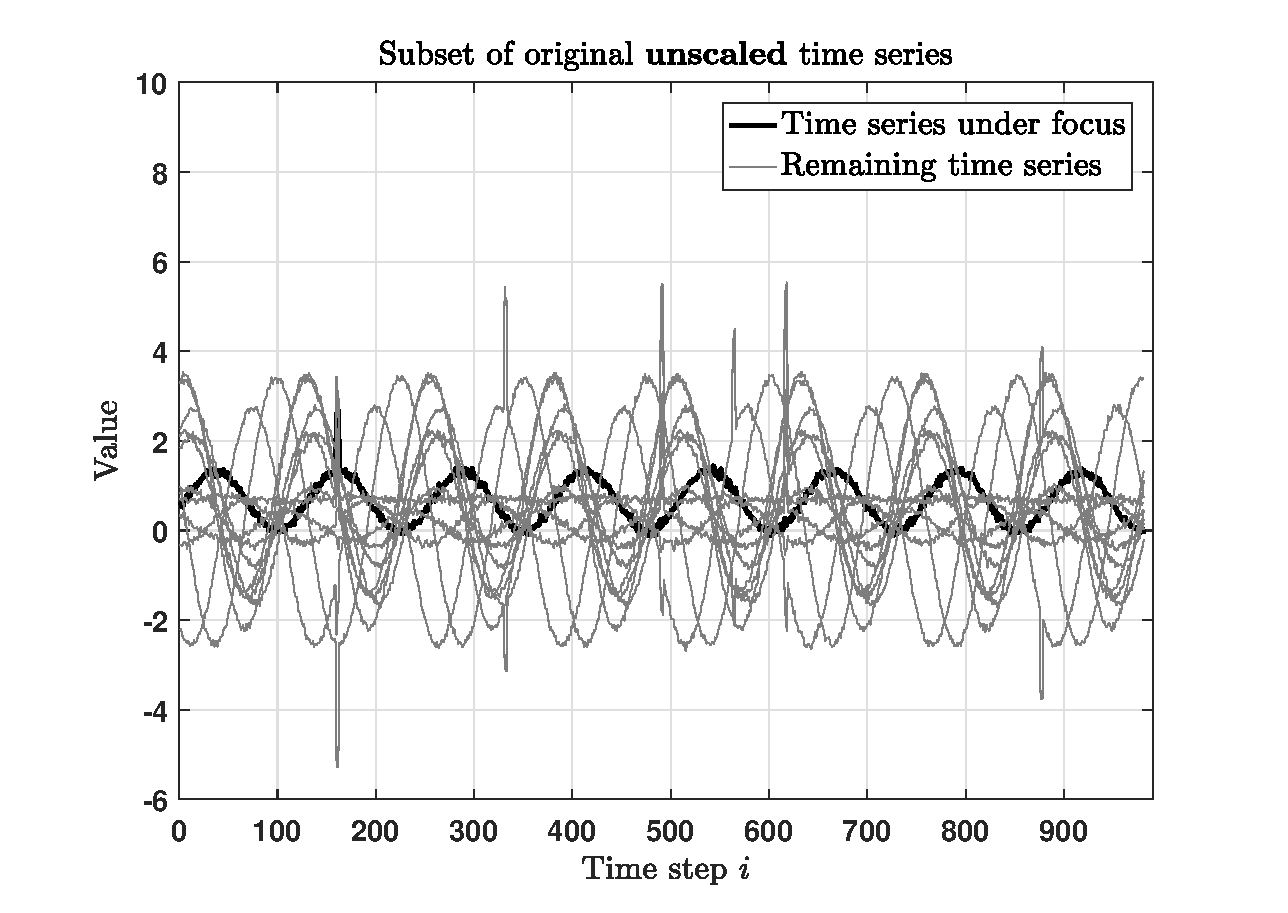
\includegraphics[scale=0.345]{analysis/Analysis_unscaled_original}
	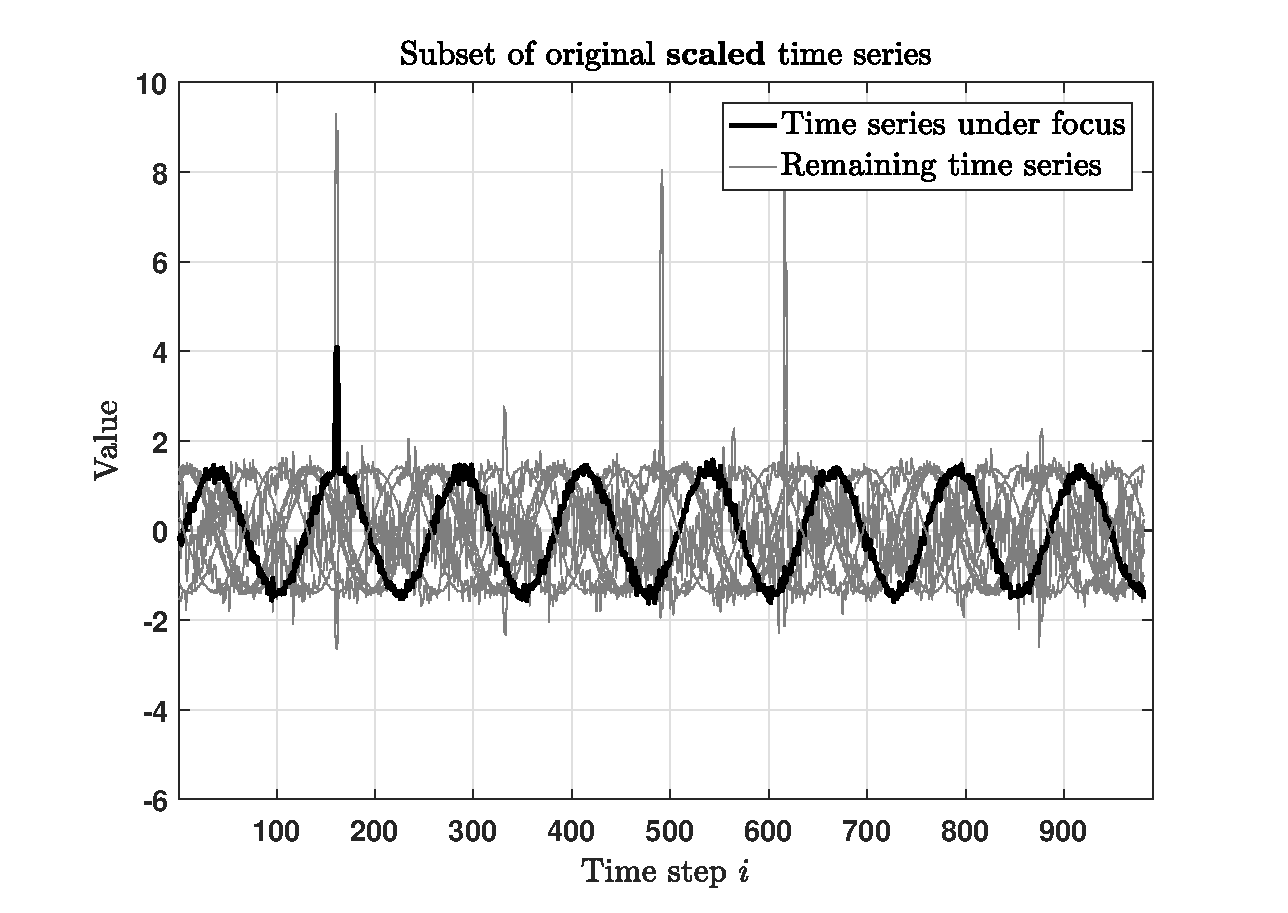
\includegraphics[scale=0.345]{analysis/Analysis_scaled_original}
	\vspace{-0.12cm}
	\caption{Original unstandardized (left) and standardized (right) subset of time series.}
	\label{fig:analysis_innerworking_original}
	\vspace{-0.1cm}
\end{figure}

Each of these $981$ $60$-dimensional data points are then projected one by one onto a $k$-dimensional projection basis, where for visualization purposes we have set $k$ to $1$ for this example. Figure \ref{fig:analysis_innerworking_projection} shows the resulting $1$D projection of the $60$D time series. 

\begin{figure}[h]
	\centering
	\vspace{-0.12cm}
	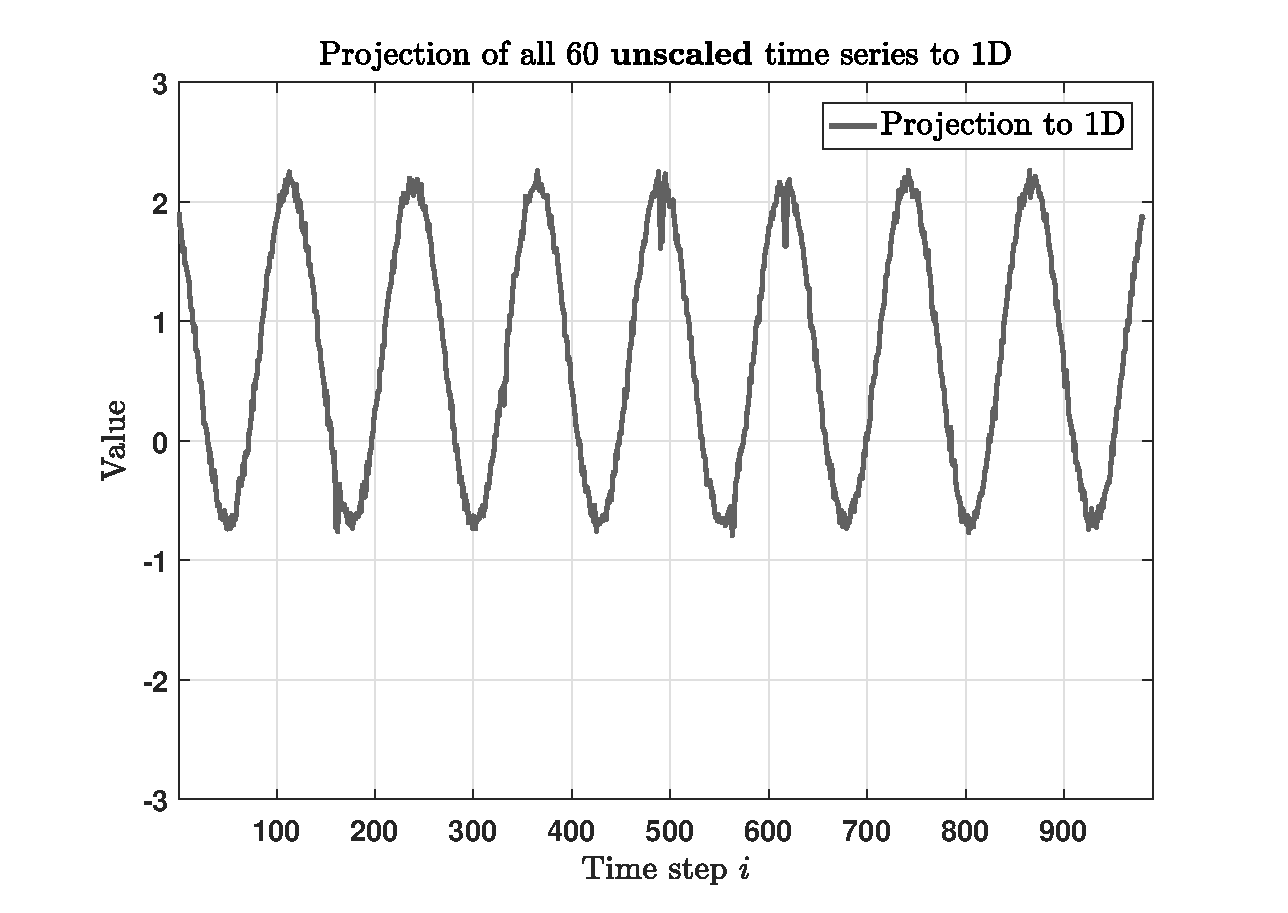
\includegraphics[scale=0.345]{analysis/Analysis_unscaled_projection}
	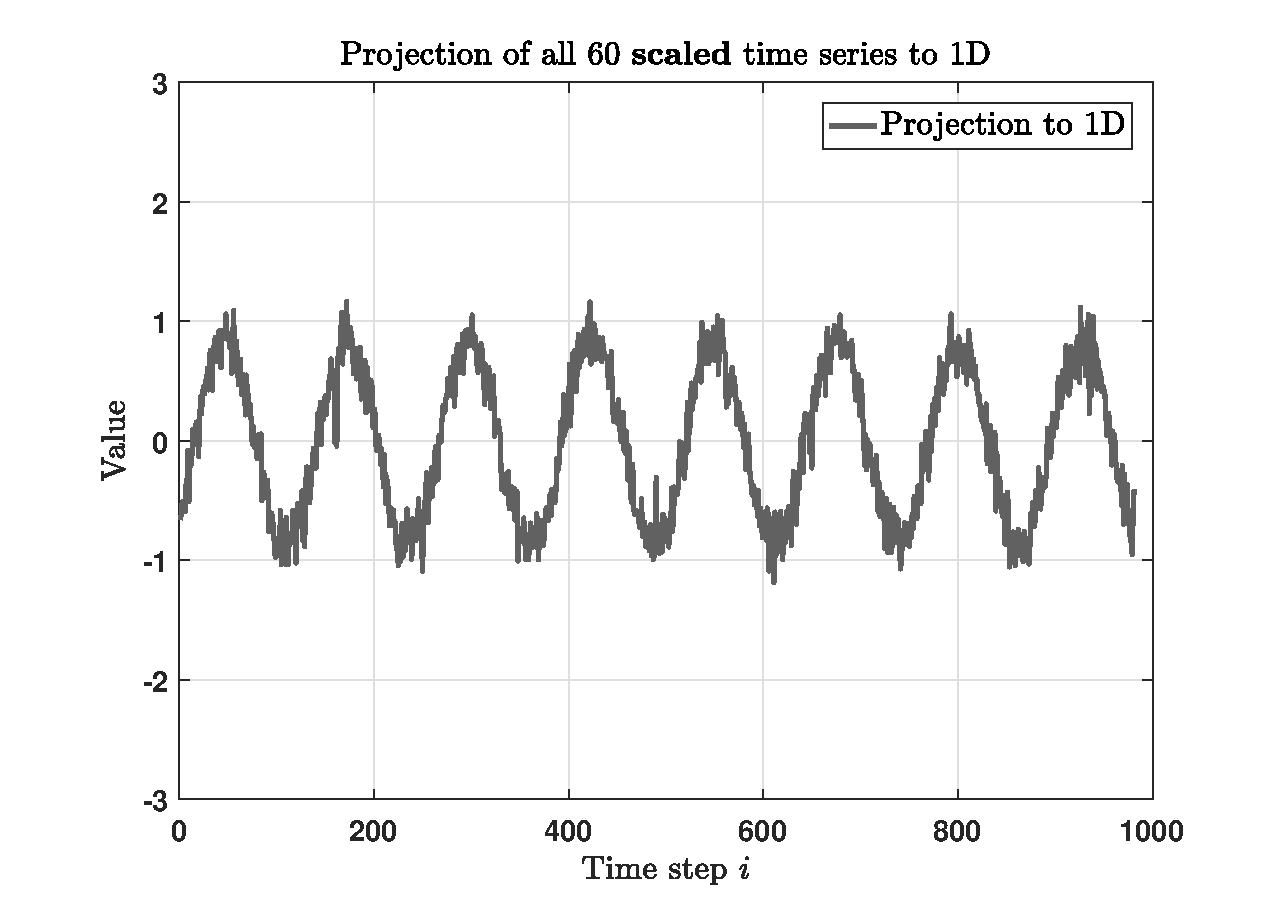
\includegraphics[scale=0.345]{analysis/Analysis_scaled_projection}
	\vspace{-0.12cm}
	\caption{Projections of the $60$D unstandardized (left) and standardized (right) time series to $1$D.}
	\label{fig:analysis_innerworking_projection}
	\vspace{-0.25cm}
\end{figure}

The principal sinusoidal behaviour can be clearly seen in both projections. We can also still see reflections of the outliers in the resulting projections at for instance $i \approx 500$. The obtained projections are reconstructed to what is shown in figure \ref{fig:analysis_innerworking_reconstruction}. Logically, the reconstructed time series all are in-phase with the $1$D projection. This causes the original time series and their reconstructions to be out-of-phase, resulting in misalignment. Again, to avoid occlusion figure \ref{fig:analysis_innerworking_reconstruction} only shows a subset of $12$ time series out of the $60$ input time series.

\begin{figure}[h]
	\centering
	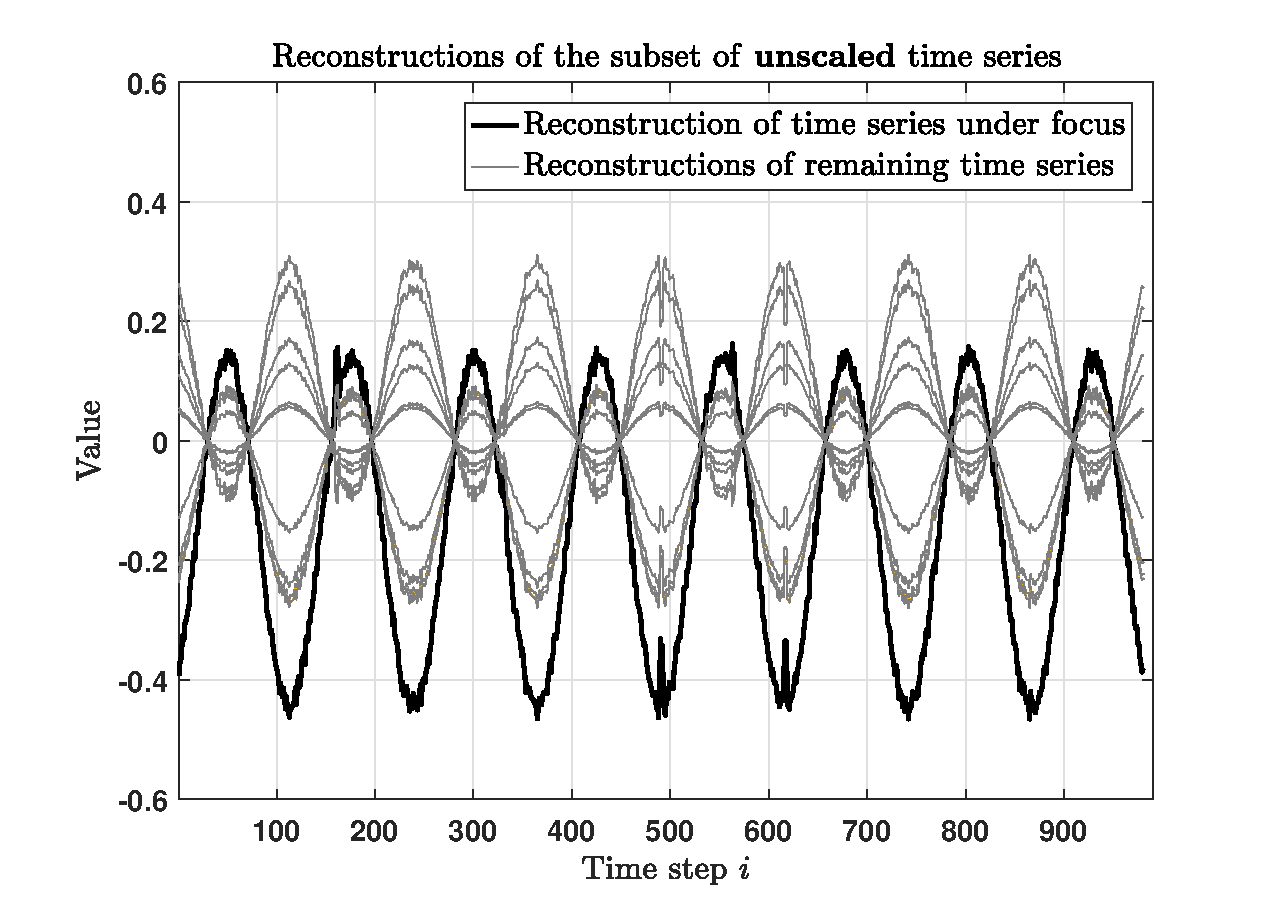
\includegraphics[scale=0.36]{analysis/Analysis_unscaled_reconstruction}
	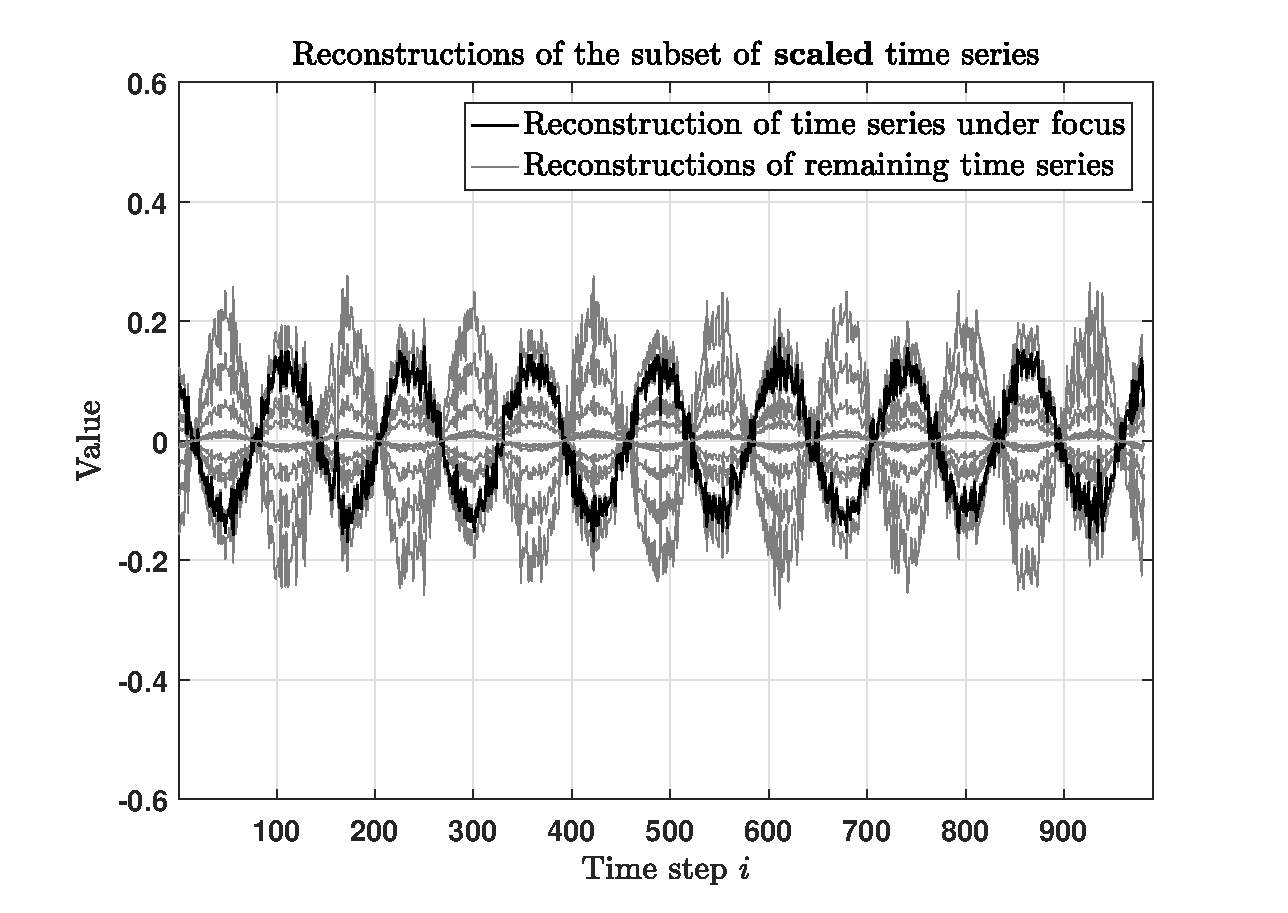
\includegraphics[scale=0.36]{analysis/Analysis_scaled_reconstruction}
	\caption{Reconstructions of unstandardized (left) and standardized (right) subset of time series.}
	\label{fig:analysis_innerworking_reconstruction}
	\vspace{-0.15cm}
\end{figure}

\newpage
The consequence of our misaligned reconstructions can be clearly recognized in the obtained outlier scores as shown in figure \ref{fig:analysis_innerworking_outlierscores}. Also note that the means of the reconstructed unstandardized time series are closer to $0$ than the means of the original time series, while the means of the reconstructed standardized time series remain $0$. Due to the larger difference in mean and range between an unstandardized time series and its reconstruction, we might be unlucky and not find the global point outliers at $i \approx \{170, 330, 570\}$, as shown at the left-hand side of figure \ref{fig:analysis_innerworking_outlierscores}. If we standardize the data we do not suffer from this as shown at the right.

\begin{figure}[h]
	\centering
	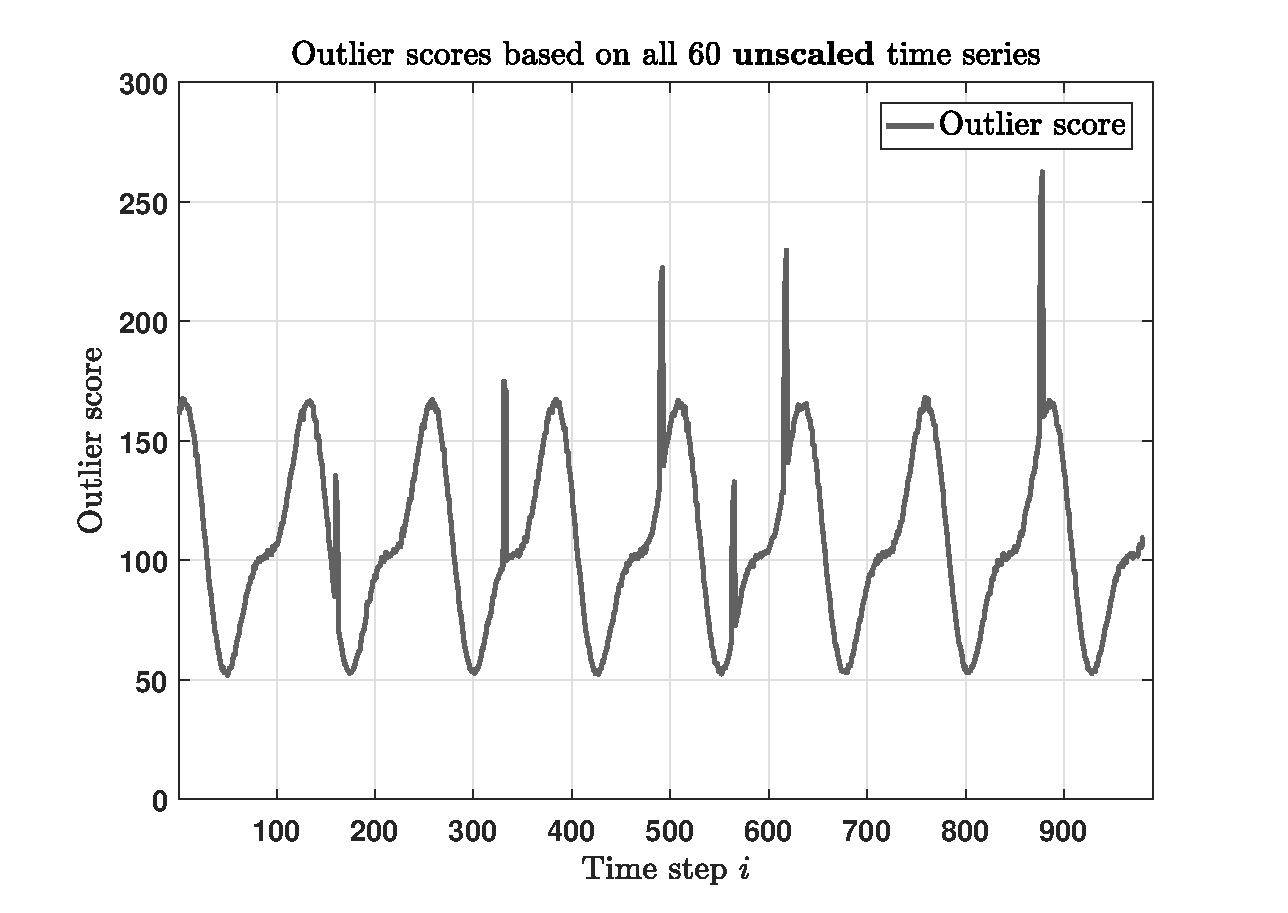
\includegraphics[scale=0.36]{analysis/Analysis_unscaled_outlierscores}
	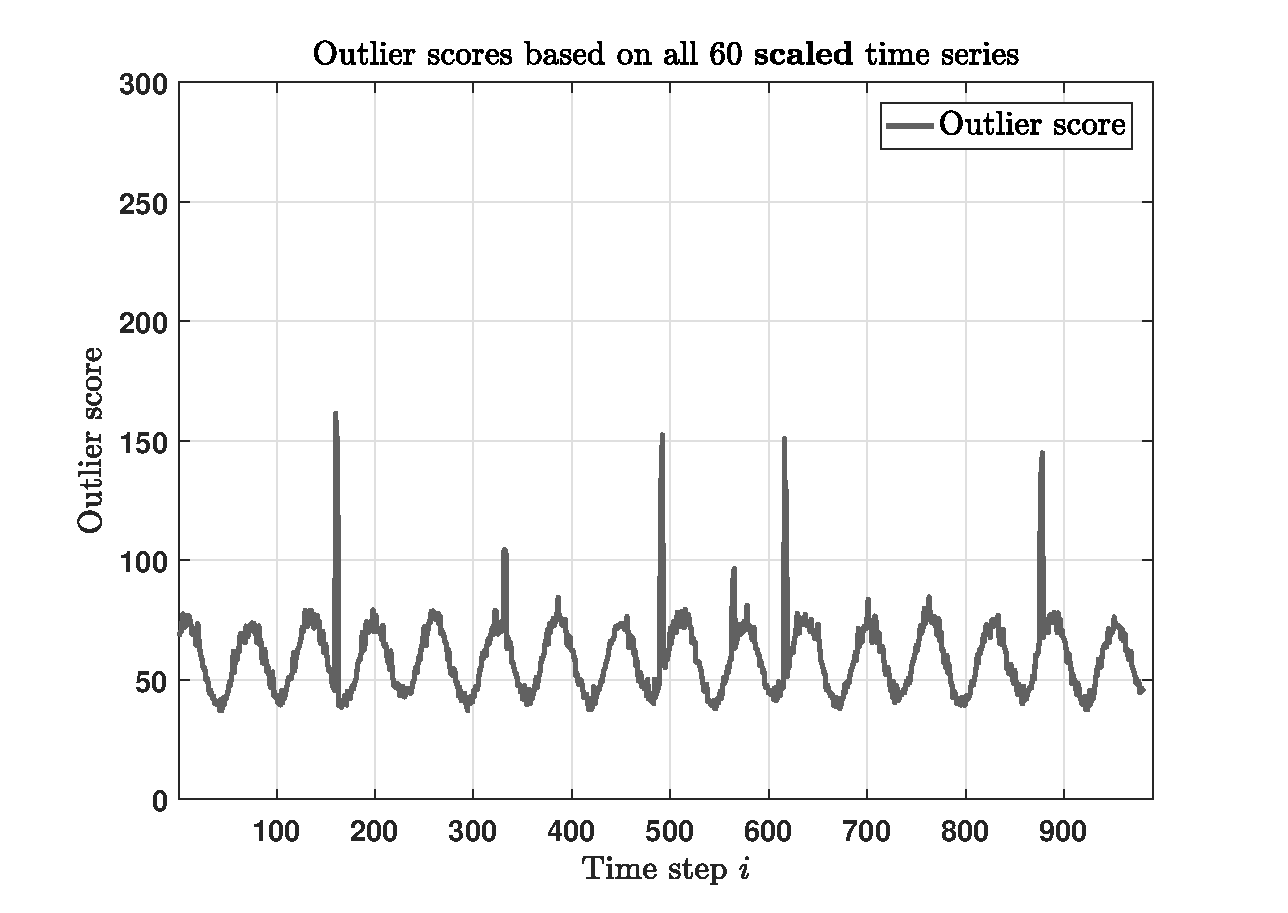
\includegraphics[scale=0.36]{analysis/Analysis_scaled_outlierscores}
	\caption{Outlier scores of unscaled (left) and scaled (right) time series.}
	\label{fig:analysis_innerworking_outlierscores}
\end{figure}

For contextual point and collective outliers we have exactly the same results up to the outlier scores. That is, due to the contextualness of these outlier types, the original time series at those time steps are likely closer to the reconstructed data points, as explained in chapter \ref{chap:rp-method}. Back-scaling in some cases resolves this problem, but certainly not always as will become clear in section \ref{sec:analysis_bird}.
Finally, it is important to realize that the RP method relies on the correlation among the different time series. To that end, the RP method does not find outliers that cause all time series to show significant deviations considering their normal behaviours. This certainly is a limitation of the method.


\section{A bird's-eye view}
\label{sec:analysis_bird}

In this section we focus on the behaviour of the detection and runtime performances of the RP method and its baseline SPIRIT under varying parameter settings. 
We investigated these behavioural properties for the $3$ different outlier types, window lengths $p = \{1,5,10,15\}$, and for the number of projection vectors $k$ from $1 \text{ to } 25$. For SPIRIT we have the forgetting factor $\lambda$ as additional parameter which we have set to $0.97$ being within the typical range of $[0.96, 0.98]$ \cite{papadimitriou2005streaming}. We also used these experiments to determine the influence of back-scaling with factor $\sqrt{\frac{d}{k}}$ on the detection performance. Therefore, we ran all experiments in this section with both versions of the RP method: with and without back-scaling. 

\begin{figure}[h]
	\centering
	\vspace{-0.1cm}
	\includegraphics[scale=0.35]{analysis/AUCs_point}
	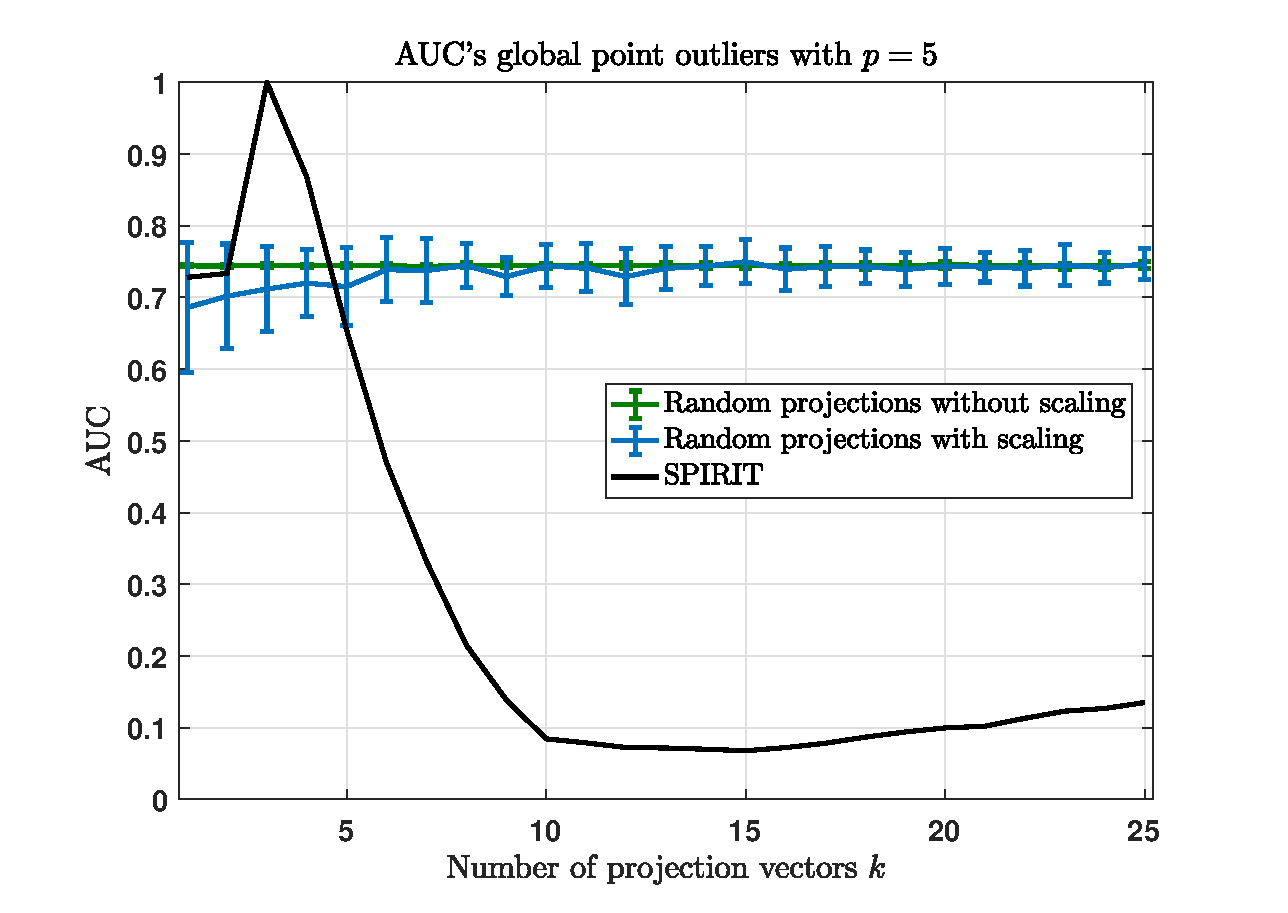
\includegraphics[scale=0.35]{analysis/AUCs_point1}\\
	\includegraphics[scale=0.35]{analysis/AUCs_point2}
	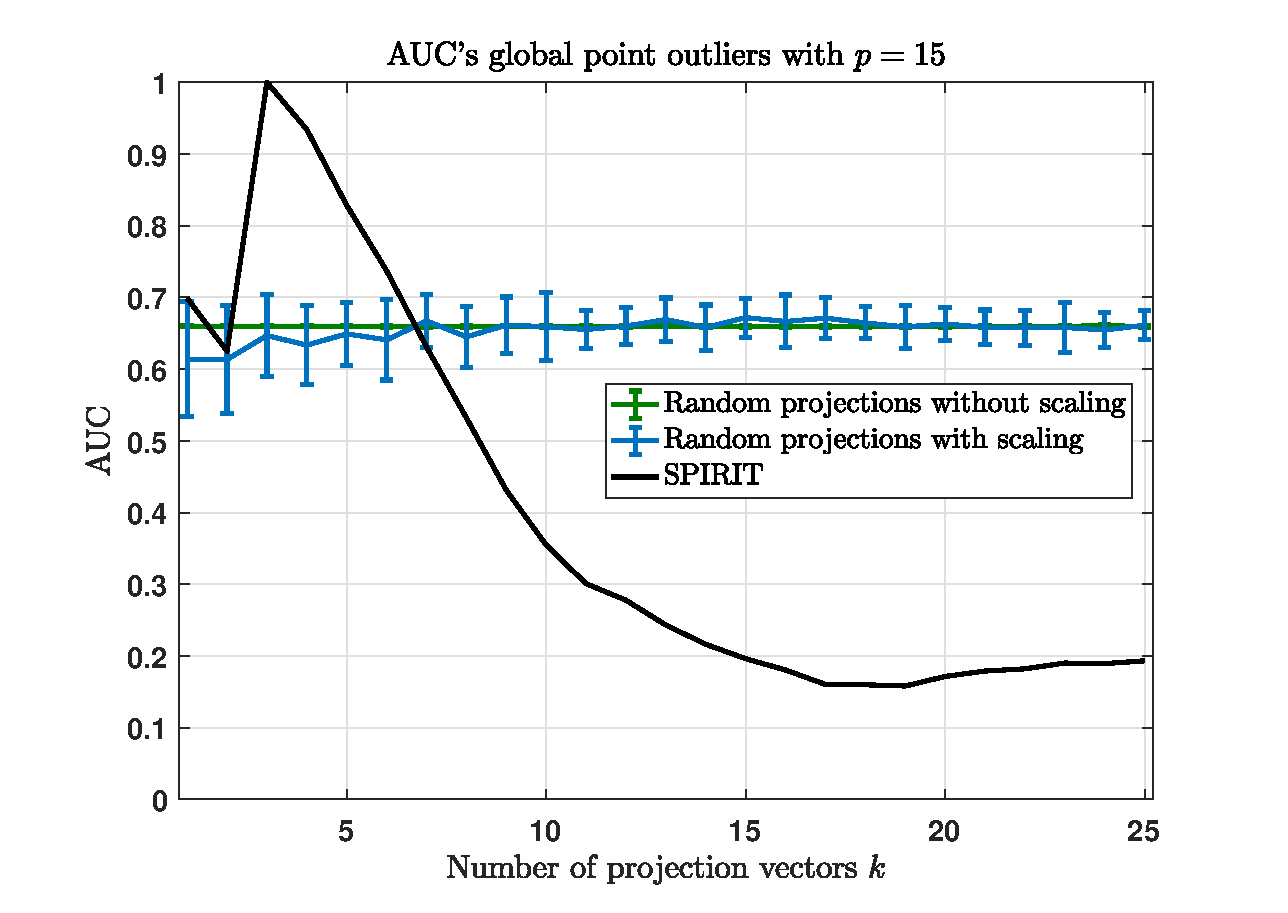
\includegraphics[scale=0.35]{analysis/AUCs_point3}
	\caption{Detection performances of global point outliers with $k$ from $1$ to $25$ and $p=\{1,5,10,15\}$.}
	\label{fig:analysis_aucs_point}
	\vspace{-0.26cm}
\end{figure}

Starting with figure \ref{fig:analysis_aucs_point}, we present the detection performances for global point outliers. It becomes clear that the AUC of SPIRIT is very sensitive to the number of projection vectors ($k$) used, as expected. SPIRIT yields a clear peak in AUC at $k=3$ where the AUC is $1$ regardless of the sliding window size, which translates to a $100\%$ chance of correctly labelling a randomly selected pair of a normal data point and an outlier. Yet the AUC drops at a high rate after adding more projection vectors. Considering the performance without a sliding window ($p=1$), the AUC even drops from $1$ to $0.1$ between $k=3$ and $k=5$ which implies that the $4^{\text{th}}$ and $5^{\text{th}}$ principal components align well with the outliers. The detection performance of the RP method with and without back-scaling is relatively insensitive to the number of projection vectors $k$ and results in an AUC around $0.9$ irrespective of $k$. The RP method without back-scaling reaches an AUC slightly higher and more stable than with back-scaling, as was expected. The RP method basically benefits from the power of the squared Euclidean distance to emphasize very large reconstruction errors (from outliers) in contrast to `just' large reconstruction errors (corresponding to normal data points).

Clearly, the advantage of stability is therefore on behalf of the random projection methods. If we would know on forehand what a proper $k$ would be for the entire stream, SPIRIT has potential to yield a very high AUC. Unfortunately it is often unknown what to expect, where the behaviour of systems is likely not as stable as our synthetic sinusoidal time series. Even if we could make an educated guess to what a sufficient value for $k$ might be, if reality deviates a little from our guess we might completely miss the principal behaviour or reconstruct our outliers better. Implementing SPIRIT with a sliding window makes the performance less sensitive to $k$, which might be sufficient to get a generally well performing method. The RP method does not benefit from a window, and even makes it perform worse.

Though we only based our expectations regarding the effects of back-scaling on loose reasoning, scaling $\hat{\mathbf{x}}_i$ back to approximate the data point its original norm results in a less stable and often worse performance compared to its not back-scaled counterpart. Another difference between the two variants of the RP method we would like to emphasize, is that the AUC of the method without back-scaling slightly decreases when more projection vectors are added in contrast to its scaled version. Throughout all (preliminary) experiments with this method, we remarkably found that for the RP method without back-scaling taking $k=1$ on average performs better than taking $k=2$ or $k=3$, etcetera, regardless of the data at hand. We elaborate on this observation in more detail in section \ref{sec:analysis_contextual}.

When it comes to comparing runtime performances, the proposed method outperforms SPIRIT heavily. Figure \ref{fig:analysis_runtimes_point} shows the runtime performances associated with the discussed detections. We are confirmed that even for $k=1$ SPIRIT runs twice as slow as the random projection method. This reveals the difference in the hidden constants behind the upper bounds on the computational complexity of the RP method and SPIRIT. That is, for $k=1$ we have no influence of the quadratic factor on the runtime of SPIRIT, yet its runtime is twice as high as from the RP method. Therefore, its upper bound is closer to $\mathcal{O}(2k^2d)$ compared to $\mathcal{O}(kd)$ of the RP method.

\begin{figure}[h]
	\centering
	\vspace{0.25cm}
	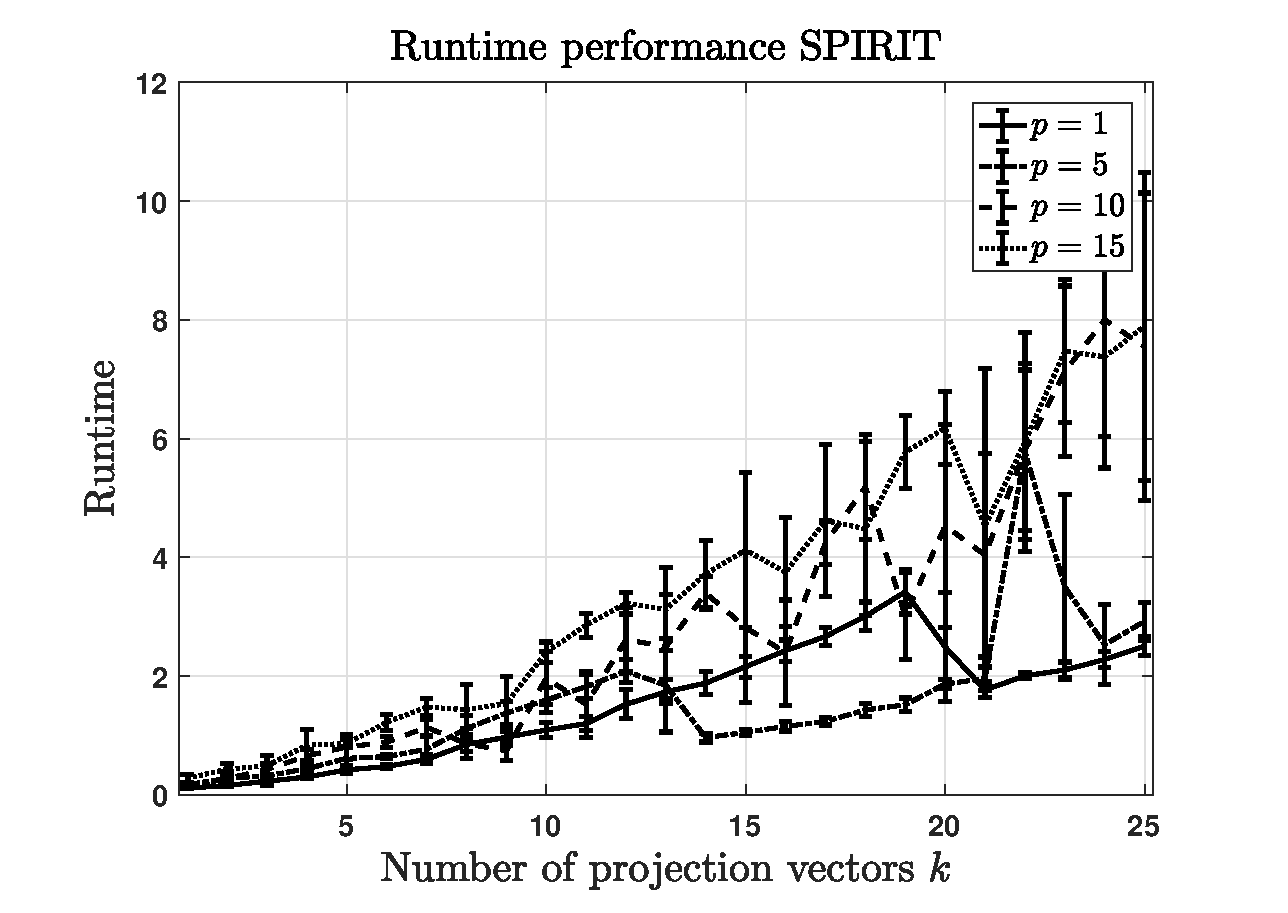
\includegraphics[scale=0.36]{analysis/Runtimes_SPIRIT_point}
	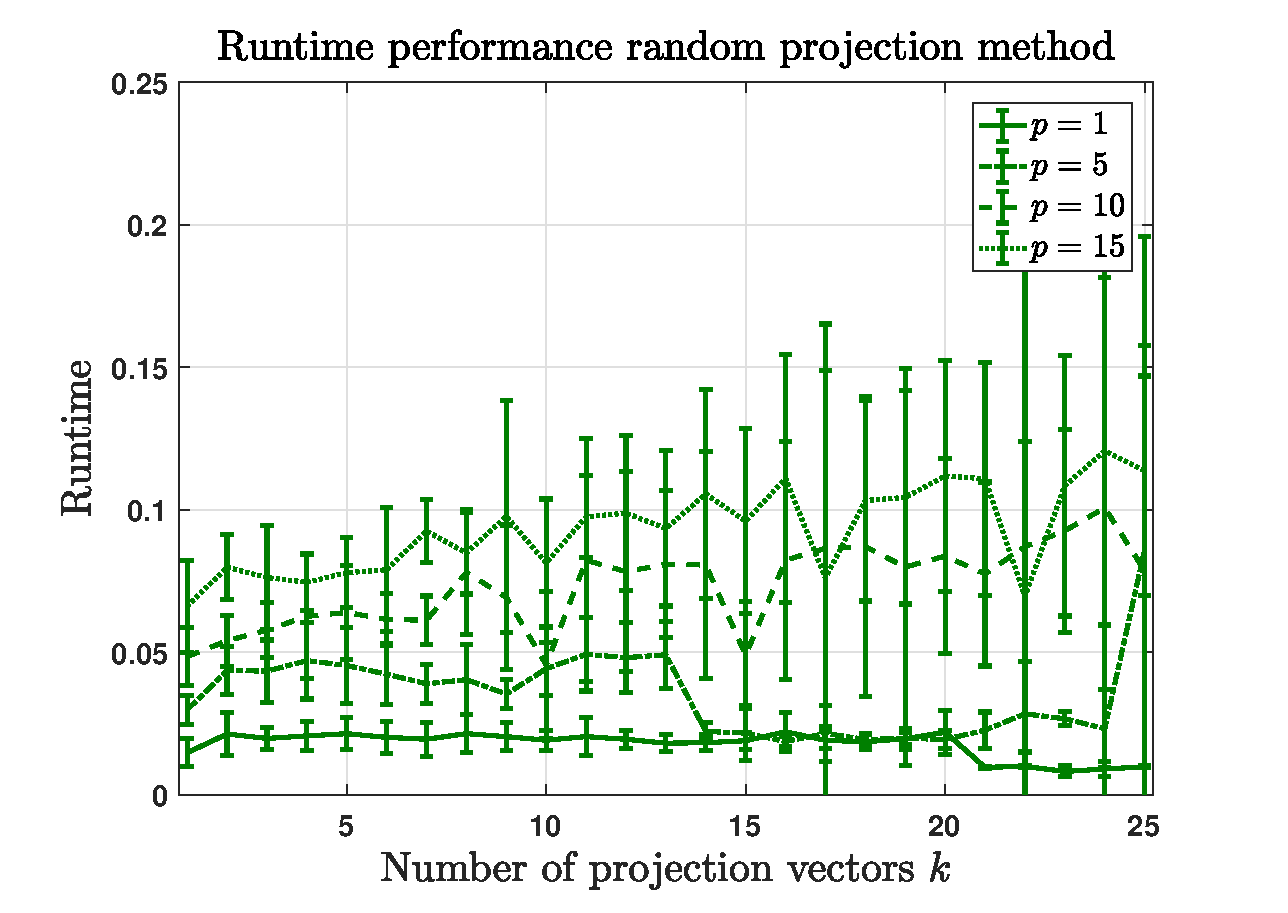
\includegraphics[scale=0.36]{analysis/Runtimes_RP_point}
	\vspace{0.1cm}
	\caption{Runtime performances of global point outliers with $k$ from $1$ to $25$ and $p=\{1,5,10,15\}$.}
	\label{fig:analysis_runtimes_point}
	\vspace{0.25cm}
\end{figure}

From figure \ref{fig:analysis_aucs_contextual} (left) it becomes clear that the RP method is less successful for finding contextual outliers. For contextual point outliers (left) it even results in stable AUC's around $0.3$, making it perform worse than random guessing the labels of a randomly selected pair of a normal data point and an outlier. Contextual collective outliers (right) are only detected a little better than random guessing. The remaining patterns compared to SPIRIT are quite similar to the observations made previously.

\begin{figure}[h]
	\centering
	\vspace{0.25cm}
	\includegraphics[scale=0.36]{analysis/AUCs_contextual}
	\includegraphics[scale=0.36]{analysis/AUCs_collective}
	\vspace{0.1cm}
	\caption{Detection performances of contextual point and collective outliers with $k$ from $1$ to $25$ for $p=1$.}
	\label{fig:analysis_aucs_contextual}
	\vspace{0.25cm}
\end{figure}

This poor performance is a direct consequence of the feature values of such outliers, which in most cases are closer to the reconstructed model than the remainder of the data points. This effect is illustrated in figure \ref{fig:analysis_contextualreconstruction} for the reconstruction with the RP method with and without back-scaling, where we used $15$ projection vectors and no sliding window. In this example the outliers are also reconstructed relatively good which is an undesired outcome as well.

\begin{figure}[h]
	\centering
	\vspace{0.1cm}
	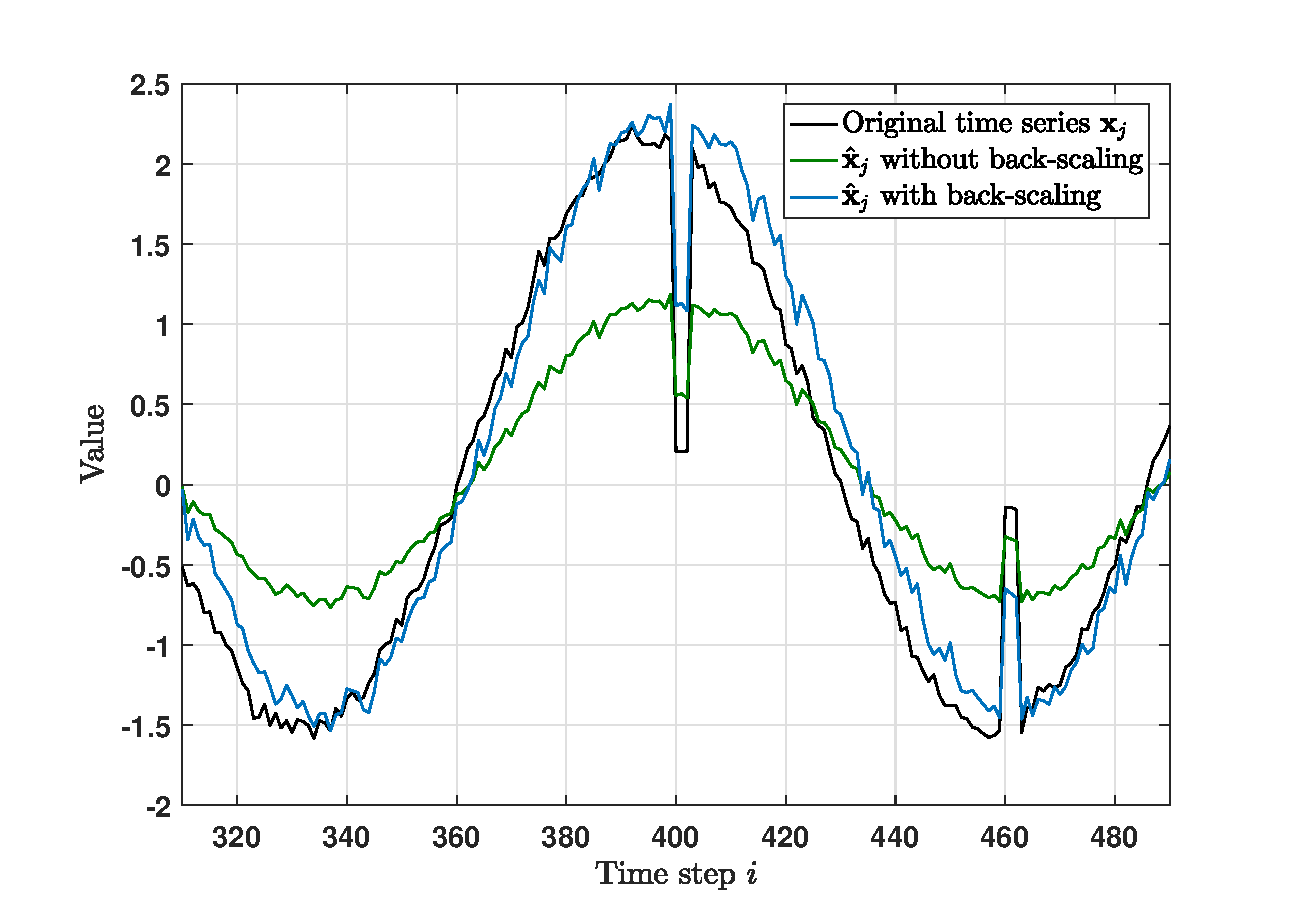
\includegraphics[scale=0.38]{analysis/Analysis_contextualreconstructionrp}
	\caption{Reconstruction of a time series with contextual outliers with $k=15$ projection vectors.}
	\label{fig:analysis_contextualreconstruction}
\end{figure}

\newpage
The squared Euclidean distances between the reconstructions of outliers and their original values are then typically smaller, resulting in reconstruction errors lower than or equal to the reconstruction errors of normal data points. Back-scaling does play an important role for finding contextual outliers as the model behaviour is then more often closer to the original behaviour, as can be derived from figure \ref{fig:analysis_contextualreconstruction} as well. However, scaling the reconstructed data point back does not significantly improve the detections which becomes clear from the AUC's in figure \ref{fig:analysis_aucs_contextual}. 

The detection performances associated with window lengths $p=\{5,10,15\}$ can be found in appendix \ref{app:analysis}. From these experiments, we found that a sliding window only helps a little for the detection of contextual outliers. Yet we need a window length $p$ of approximately $15$ data points to obtain an AUC around $0.5$ for contextual point outliers. As the runtime performances are independent of the type of outliers in the data, the runtime performances are similar to what has been shown in figure \ref{fig:analysis_runtimes_point} and therefore are not presented.

With or without back-scaling and adopting a sliding window or not, deriving outlier scores from reconstructions from random projections does not have a high potential for contextual outliers. \\

\noindent In short, we observed the following from this analysis:
\begin{itemize}
	\itemsep-0.2em
	\item The RP method performs competitive AUC-wise when the outliers are global, but SPIRIT is more successful in finding outliers of all three types.
	\item The RP method without back-scaling results in a less accurate model of the original data but yields a more stable performance for all outlier types. The back-scaled version, however, is slightly better at detecting contextual outliers.
	\item The detection performance of the RP method is stable for varying number of projection vectors $k$ and often obtains its optimal performance for $k=1$. Therefore, taking $k=1$ would be a generally safe option making this method parameter-free.	
	\item The detection performance of SPIRIT is highly sensitive to the number of projection vectors $k$.
	\item The RP method does not benefit from a window and by default does not exploit temporal relations over time. 
	\item SPIRIT benefits from a window as it reduces its sensitivity of the detection performance to $k$.
	\item The runtime of the RP method is low and only linearly depending on $k$.
	\item SPIRIT is tractable if the data is highly correlated or low dimensional due to the low number of projection vectors needed in those cases. If more vectors are needed to explain the desired variance, this method becomes expensive as its runtime quadratically depends on $k$.
\end{itemize}

Two observations are particularly interesting: the RP method yields very poor results for contextual outliers, but reaches its optimal operating point for $k=1$. In the next section we elaborate more on these conclusions.


\section{Detecting contextual outliers}
\label{sec:analysis_contextual}

Contextual outliers are most often misclassified if we assign outlier scores as in algorithm \ref{alg:analysis_algorithm}. This is caused by the feature values of such outliers, which are closer to the values of the reconstructed data point. This results in a lower reconstruction error than for normal data points, hence resulting in AUC's lower than $0.5$. Missing them can be critical for outlier detection in multivariate time series as contextual outliers might appear in the data.

One solution to detect the contextual point outliers more accurately is by taking the inverse of the outlier scores ($\frac{1}{O_i}$) such that the labels are reversed. Doing so would not significantly affect the runtime performance. However, it would obviously not be effective for finding global point outliers, or contextual collective outliers for which the AUC's then will be lower than $0.5$. We could take the maximum of the combination of the original outlier scores and their inverses instead. Unfortunately, we would not get an AUC higher than around $1 - 0.3 = 0.7$ this way for contextual point outliers.

Another observation was that we often detect outliers better with only one projection vector than when we use multiple, regardless of the type of outliers. That is, the RP method yields on average its optimal AUC with $k=1$ and therefore is higher than with $k=1+\Delta$.
Recall, that we assign outlier scores directly from reconstruction errors. Linking this to our observation, it can be concluded that we can separate outliers from normal data points worse by their reconstruction errors, when we increase the number of projection vectors $k$. This would imply that the outliers are reconstructed better at a faster rate than normal data points are after adding a random projection vector to the projection matrix. 
This brings us to the formulation of hypothesis \ref{hyp:analysis_outlierinlier}.


\begin{hypothesis}\label{hyp:analysis_outlierinlier}
	For $k, \Delta > 0$, let $\mathbf{X}$ be an arbitrary data set of size $d \times n$ with sufficiently correlated features.
	Then with high probability we have for all $\mathbf{x} \in \mathbf{X}$:

	\[ |\mathcal{E}_{k,\text{normal}} - \mathcal{E}_{k+\Delta,\text{normal}}| \ < \ |\mathcal{E}_{k,\text{outlier}} - \mathcal{E}_{k+\Delta,\text{outlier}}| \]
	
	\vspace{0.2cm}
	
	\noindent with $\mathcal{E}_{k,\mathbf{x}}$ the reconstruction error of data point $\mathbf{x}$ obtained with the RP method.
\end{hypothesis}

Though it would be interesting to formally prove hypothesis \ref{hyp:analysis_outlierinlier}, in this thesis we focus on exploiting it to find contextual outliers besides global outliers. But, how can we do this?
Going back to the fundamental objective of outlier detection methods, we aim at assigning higher outlier scores to outliers than to normal data points. Such a relation between normal data points and outliers follows directly from our hypothesis. If hypothesis \ref{hyp:analysis_outlierinlier} holds and we compute the outlier scores as 

\begin{equation}\label{eq:hypothesis_outlierscores}
	O_i \gets |\| \mathbf{x}_i - \hat{\mathbf{x}}_i \|^2_{k} - \| \mathbf{x}_i - \hat{\mathbf{x}}_i \|^2_{k+\Delta}|,
\vspace{0.1cm}
\end{equation}

\noindent we would get higher outlier scores for outliers than for normal data points.\\
Unfortunately, this introduces two drawbacks. First, we might end up projecting in such a way that we reconstruct our outliers better which happens with an unknown probability. To avoid these occurrences we can rely on taking the maximum of $m$ distinct predictions for $O_i$. Sadly, this introduces a parameter, $m$ the number of predictors and increases the runtime. 

Second, the resulting reconstruction errors are likely in a different range. This issue can be resolved by standardizing the reconstruction errors obtained with $k$ and $k+\Delta$ projection vectors. By standardizing the outlier scores of the predictors, they get $0$ mean and unit variance. It is not tractable to keep a large window of the stream in memory to compute the mean and standard deviation at each time step $i$, which also would introduce this window length as an additional parameter. Therefore, we only track a few scalars estimating these statistics following equations \eqref{eq:analysis_online_mean} to \eqref{eq:analysis_online_std}, for which thorough derivations can be found in \cite{finch2009incremental}.


\begin{equation}\label{eq:analysis_online_mean}
	\mu_i = \mu_{i-1} + \frac{\mathbf{z}_i - \mu_{i-1}}{i}
\end{equation}

\begin{equation}\label{eq:analysis_online_var}
	S_i = S_{i-1} + (\mathbf{z}_i - \mu_{i-1}) \ (\mathbf{z}_i - \mu_i)
\end{equation}

\begin{equation}\label{eq:analysis_online_std}
	\sigma_i = \sqrt{\frac{S_{i}}{i}}
\end{equation}

Note, that these equations only reflect the estimation of the mean and standard deviation of one outlier score vector $\mathbf{z}$ over time. However, we also need to standardize the set of $m$ predictions for each data point over time ($\mathbf{O}_{\text{stand},m}$), so we have $m$ such means and standard deviations for this set over time. We refer to the low-cost online standardization procedure as stand($\mathbf{z}_i$). The resulting adjusted interpretation of outlier scores generated by the RP method is summarized in algorithm \ref{alg:analysis_algorithm_delta}. We refer to this interpretation as $\Delta$RP.

\vspace{-0.2cm}	
\begin{algorithm}[H]
	\caption{\quad \textbf{$\Delta$RP}}
	\label{alg:analysis_algorithm_delta}
	\begin{flushleft}
	\vspace{-0.2cm}
	\textbf{Input} data point $\mathbf{x}_i$ of size $d \times 1$\\
	\textbf{Input} number of predictors $m$	
	\vspace{-0.1cm}
	\end{flushleft}
	\begin{algorithmic}[1]	
		\vspace{-0.2cm}
		\STATE Initialize set of predictors $\mathbf{O}_{\text{stand},m}$ as $\emptyset$
		\FOR{$j$ in $m$ predictors}
			\STATE $O_{1,j} \gets \text{RP}(\mathbf{x}_i, k=1)$
			\STATE $O_{2,j} \gets \text{RP}(\mathbf{x}_i, k=2)$
			\STATE Add $\text{stand}(|\text{stand}(O_{1,j}) - \text{stand}(O_{2,j})|)$ to $\mathbf{O}_{\text{stand},m}$
		\ENDFOR
		\STATE $O_i = \max \{\mathbf{O}_{\text{stand},m}\}$
	\end{algorithmic}
	\begin{flushleft}
	\vspace{-0.3cm}
	\textbf{Output} outlier score $O_i$
	\vspace{-0.3cm}
	\end{flushleft}
\end{algorithm}
\vspace{-0.2cm}

As we are particularly interested in the detection performance of $\Delta$RP with respect to contextual outliers, we illustrate the inner working of this method by means of the data with contextual point outliers. Again, we only show a subset of $12$ time series instead of all $60$ time series to avoid occlusion. Figure \ref{fig:analysis_example_original} shows the time series we focus on throughout this example in the context of these $12$ time series.

\begin{figure}[h]
	\centering
	\vspace{-0.15cm}
	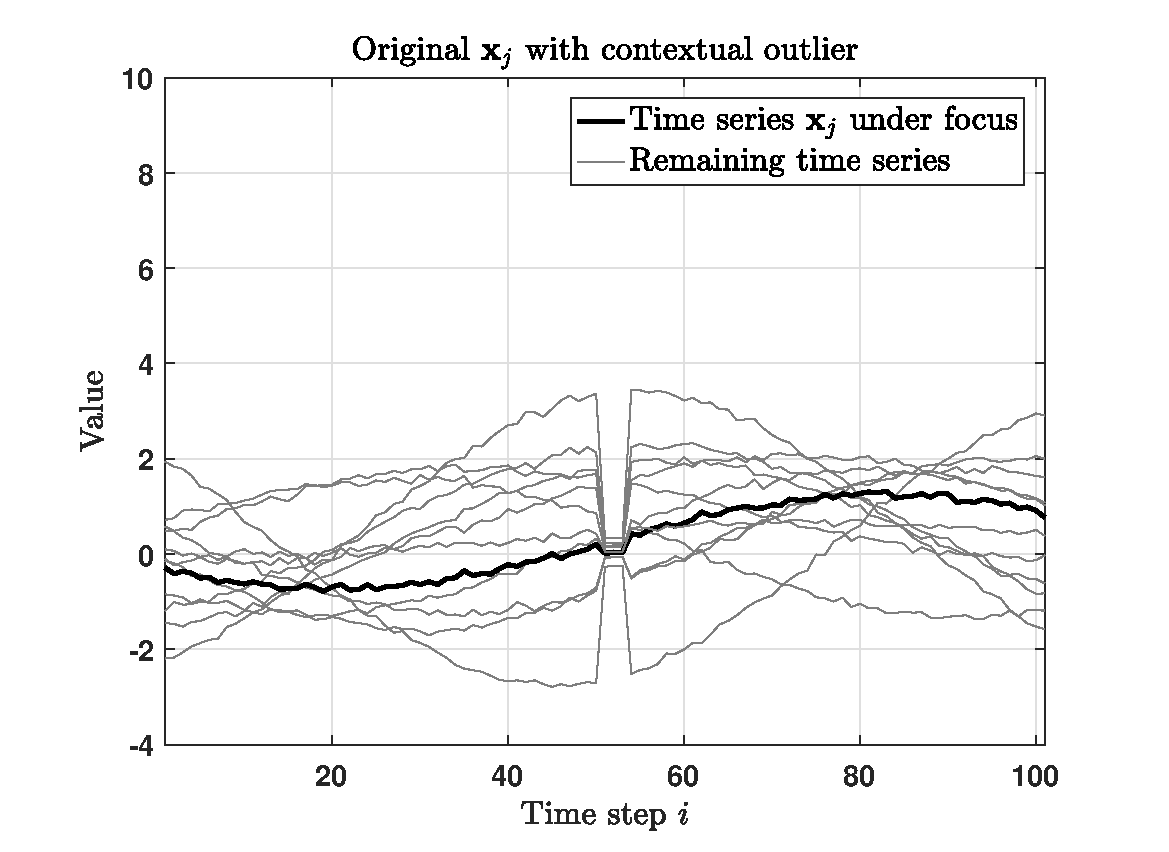
\includegraphics[scale=0.35]{analysis/Analysis_deltarp_original}
	\caption{Original subset of time series with contextual outliers.}
	\label{fig:analysis_example_original}
	\vspace{-0.15cm}
\end{figure}

The original $60$ time series are then projected once into $1$ and once into $2$ random directions with the default RP method as formulated in algorithm \ref{alg:analysis_algorithm}. Figure \ref{fig:analysis_example_projections} shows the resulting $1$D (left) and $2$D projection (right). The figure corresponding to the projection with $k=2$ (right) illustrates how projecting the data into two approximately orthogonal directions likely yields a better reconstruction of the outliers than when projecting in only $1$ random direction. 

\begin{figure}[h]
	\centering
	\vspace{-0.15cm}
	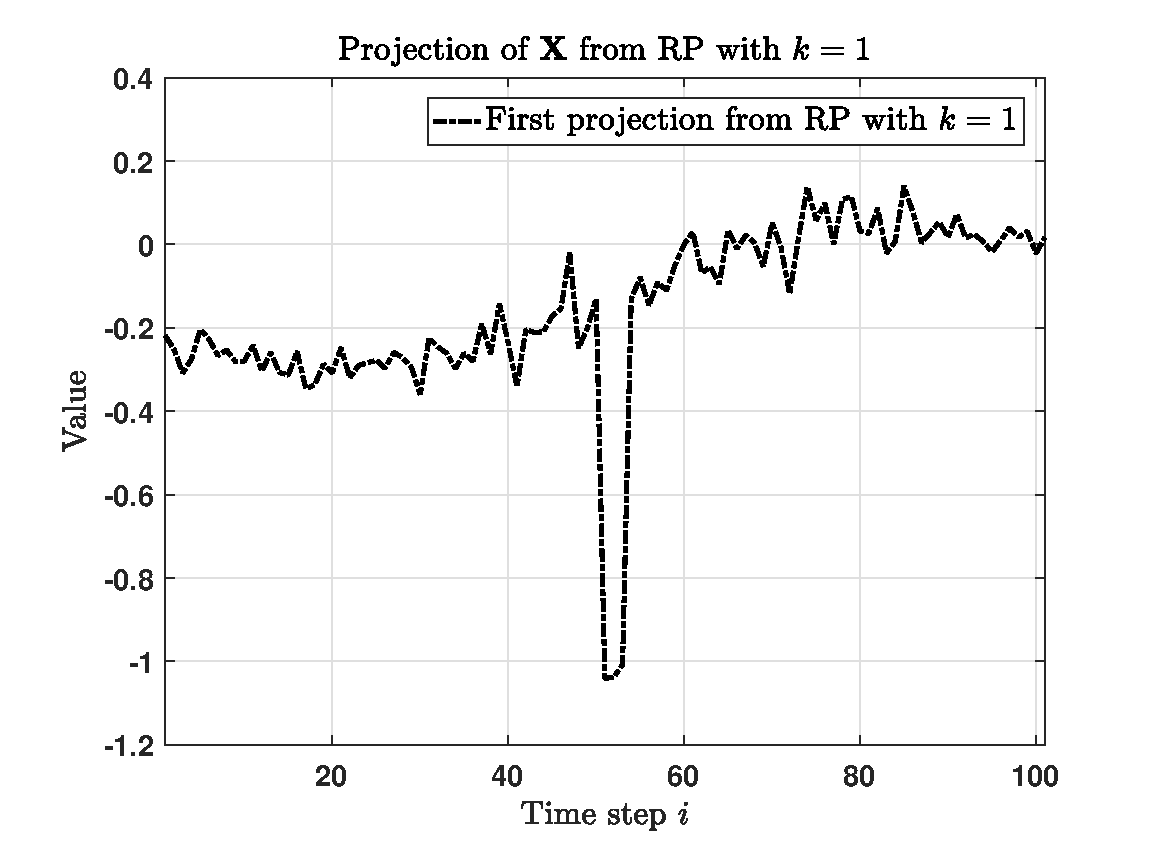
\includegraphics[scale=0.35]{analysis/Analysis_deltarp_projection1}
	\includegraphics[scale=0.35]{analysis/Analysis_deltarp_projection2}
	\caption{Projections of RP with $k=1$ (left) and $k=2$ (right).}
	\label{fig:analysis_example_projections}
	\vspace{-0.3cm}
\end{figure}

Figure \ref{fig:analysis_example_reconstructions} (left) shows what happens when we reconstruct the projections from the $1$D and $2$D projections. Despite the misalignment caused by the distinct random directions, it becomes clear that the reconstruction of the outlier around $i=500$ with $k=2$ is much closer to the original data point compared to $k=1$ which shows a high peak around $i=500$. This in turn results in a larger absolute difference between the two reconstructions of the outlier obtained with $k=1$ and $k=2$ than between the reconstructions of the normal data points surrounding this outlier (right). 

\begin{figure}[h]
	\centering
	\vspace{0.15cm}
	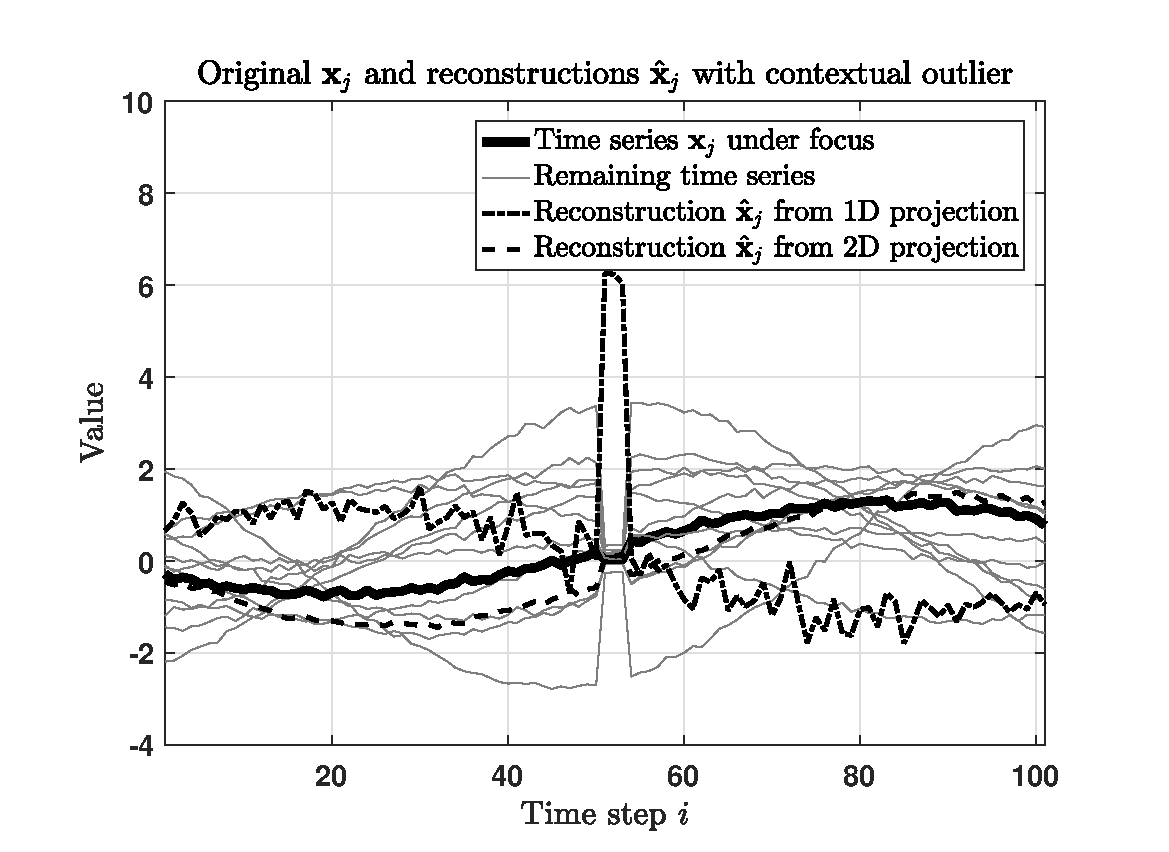
\includegraphics[scale=0.36]{analysis/Analysis_deltarp_original_reconstructions}
	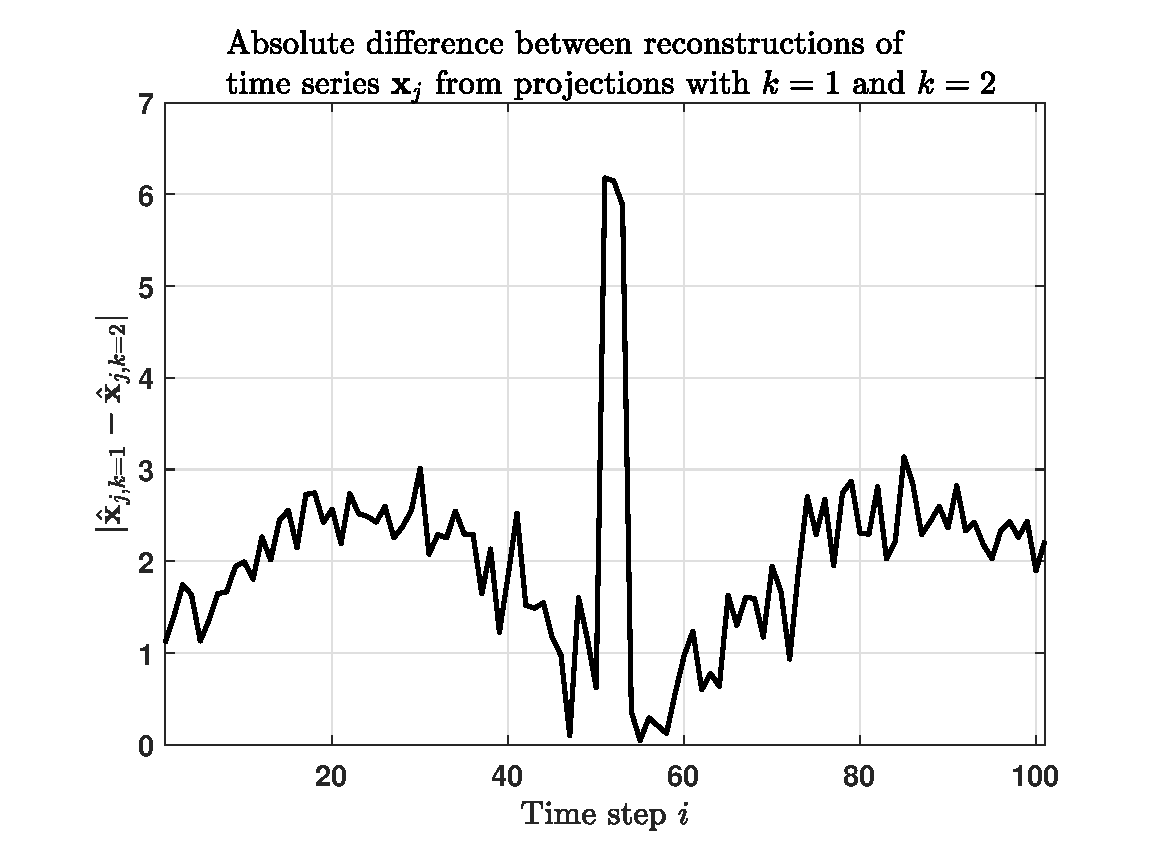
\includegraphics[scale=0.36]{analysis/Analysis_deltarp_diffreconstructions}
	\caption{Example reconstructions of time series with $k=1$ and $k=2$ (left) and corresponding absolute difference (right).}
	\label{fig:analysis_example_reconstructions}
	\vspace{0.15cm}
\end{figure}

As we have one (other) parameter to set for $\Delta$RP, $m$ the number of predictors for $O_i$, we can observe its performance for $m$ from $1$ to $25$ against SPIRIT for which we observe its performance for the number of projection vectors $k$ from $1$ to $25$ as well. This analysis has also been conducted on the standardized data of which the results are presented and discussed in appendix \ref{app:analysis}. Figure \ref{fig:analysis_aucs_global_spiritdelta} shows the results of the experiments for detecting global point outliers.

\begin{figure}[h]
	\centering
	\vspace{0.15cm}
	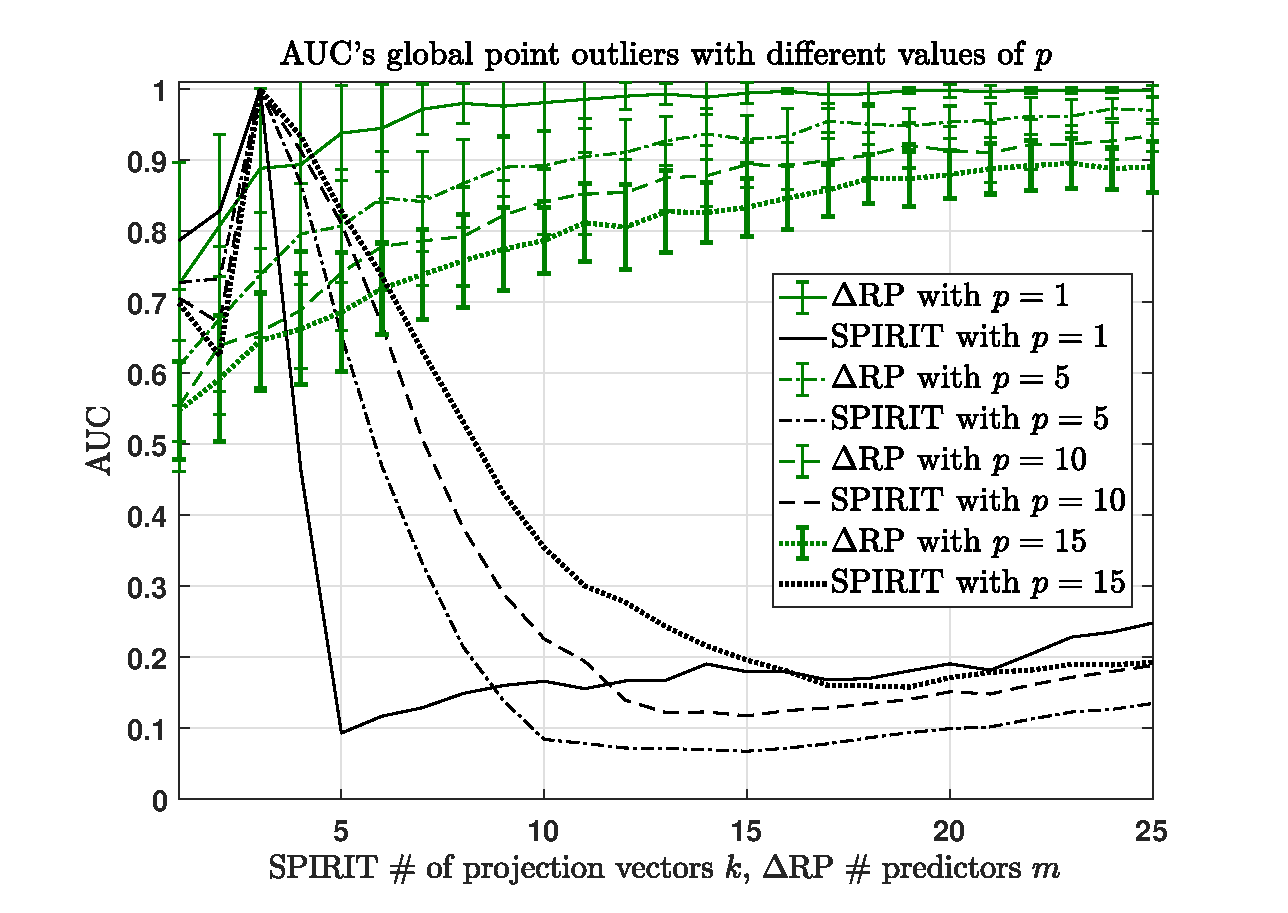
\includegraphics[scale=0.36]{analysis/AUCs_point_spiritdelta}
	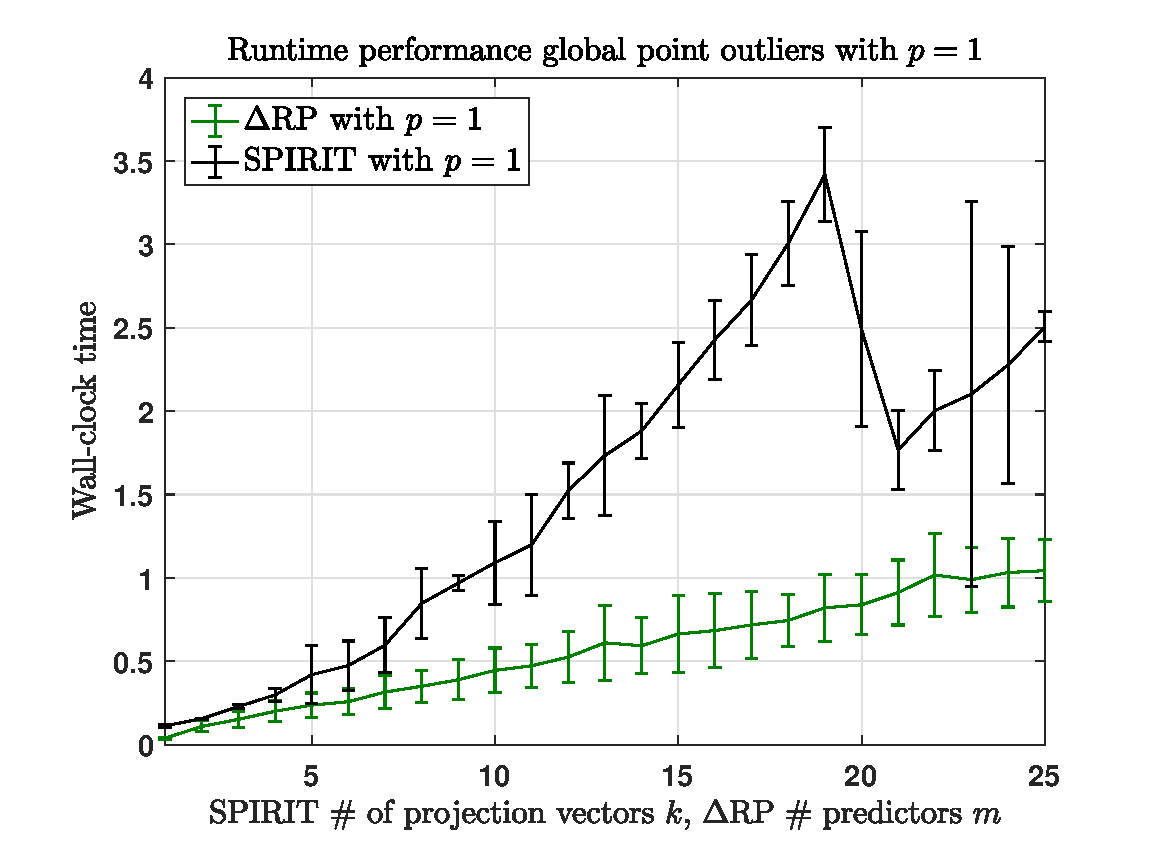
\includegraphics[scale=0.38]{analysis/Runtimes_point_spiritdelta}
	\caption{Detection and runtime performances of global point outliers with $k$ and $m$ from $1$ to $25$ for $p=\{1,5,10,15\}$.}
	\label{fig:analysis_aucs_global_spiritdelta}
	\vspace{-0.1cm}
\end{figure}

Comparing these performances with the results as shown in figure \ref{fig:analysis_aucs_point}, it can be concluded that $\Delta$RP yields, on average, a better detection performance than following the RP method as in algorithm \ref{alg:analysis_algorithm}.
For this data set we do need a relatively large number of predictors to approach the optimal performance of SPIRIT. However, $\Delta$RP likely outperforms SPIRIT when deployed in online mode as the accurate number of projection vectors $k$ is unknown on forehand, while SPIRIT its detection performance is very sensitive to $k$ and thus to the variance bounds.

Similar to the previous observations, the RP-based methods perform best without a window as its optimal performance is, again, achieved for $p=1$. The performance of $\Delta$RP can be considered more sensitive than RP as it depends on $m$ what AUC is achieved. However, if we would take $m \geq 5$ we would at least have an AUC of approximately $0.95$ on average with a relatively small standard deviation, while the performance of SPIRIT can be deteriorated if unlucky guesses for its parameters are made. 

\newpage
The key point of our interest is the performance of $\Delta$RP regarding contextual outliers. The detection performances of the experiments for contextual point and collective outliers are shown in figure \ref{fig:analysis_aucs_contextual_spiritdelta}. Since the sizes of the data sets are the same, the runtime performances are comparable to what is already presented in figure \ref{fig:analysis_aucs_global_spiritdelta}.

\begin{figure}[h]
	\centering
	\vspace{-0.05cm}
	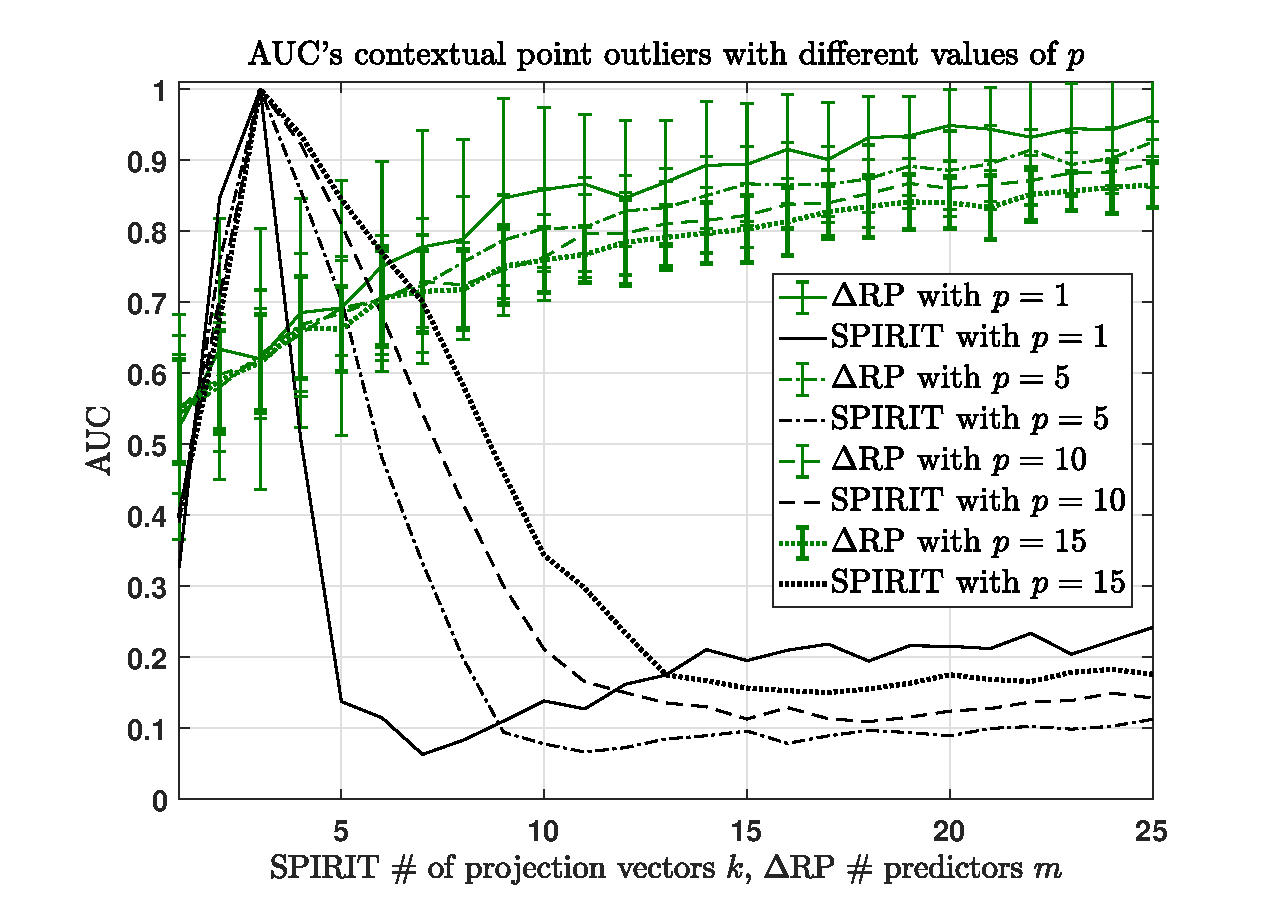
\includegraphics[scale=0.36]{analysis/AUCs_contextual_spiritdelta}
	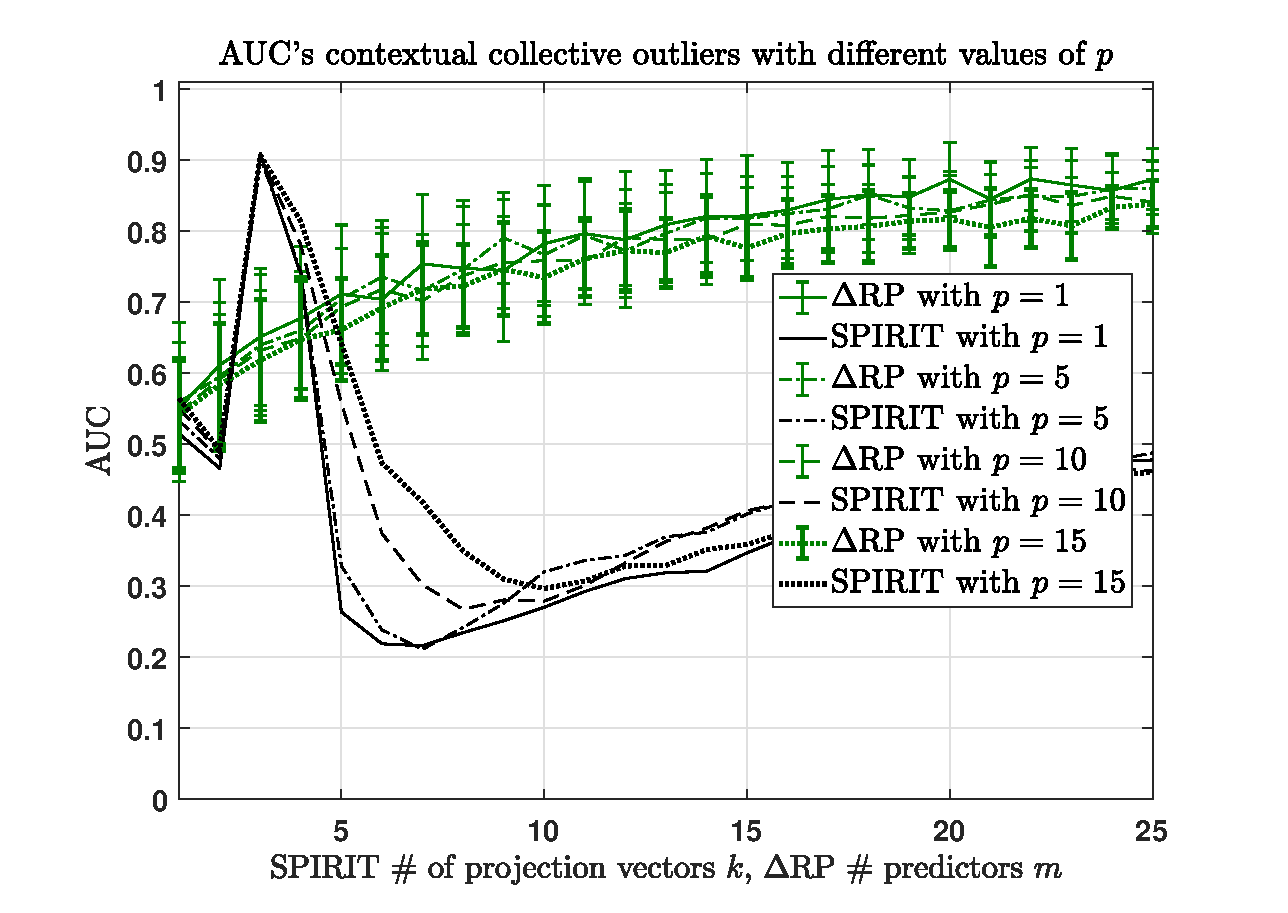
\includegraphics[scale=0.36]{analysis/AUCs_collective_spiritdelta}
	\caption{Detection performances of contextual point and collective outliers with $k$ and $m$ from $1$ to $25$ for $p=\{1,5,10,15\}$.}
	\label{fig:analysis_aucs_contextual_spiritdelta}
	\vspace{-0.05cm}
\end{figure}

We can conclude that the random projection method detects contextual outliers much better when comparing the outlier scores from runs with RP for $k=1$ and $k=2$ than the RP method. Only for the contextual outliers we possibly need a larger set of predictors to approach the optimal performance of SPIRIT. However, it is less sensitive to the number of predictors $m$ than SPIRIT is to the number of projection vectors $k$.


\section{RP and \texorpdfstring{$\Delta$RP}{deltaRP} in online mode}
\label{sec:analysis_worm}

The experiments presented so far led to interesting observations regarding the potential and parameter-sensitivity of the RP method, $\Delta$RP and SPIRIT. In this section, we focus on the online performance of these methods under realistic and fixed parameters. This analysis has also been conducted for standardized data of which the results are presented and discussed in appendix \ref{app:analysis}.

To observe the performance of the methods in online mode, we deploy SPIRIT in its adaptive mode which approximates the number of principal components needed to explain most of the variance online. This requires lower and upper bounds with respect to the explained variance that guide this online adaptation of the number of components. For adaptive SPIRIT, we followed the suggestions from the original paper \cite{papadimitriou2005streaming} for $f_{\hat{E}}$ and $F_{\hat{E}}$. The suggested bounds also resulted in a relatively good detection performance while not being too tight and, therefore, biased towards the data sets. The RP method is deployed with $1$ projection vector, $k=1$, and for $\Delta$RP we present the results for $m=5$ to ensure it has a competitive runtime performance compared to SPIRIT. We did not apply a sliding window such that $p=1$ for all three methods. Table \ref{tab:analysis_parameters} summarizes these parameter settings. 

\begin{table}[h]
	\centering
	\caption{Parameter settings for the analysis in online mode.}
	\label{tab:analysis_parameters}
	\vspace{-0.05cm}
	\begin{tabular}{l c c}
		\toprule	
		\textbf{Method}					& \textbf{Parameter}		& \textbf{Value}		\\
		\midrule
		\multirow{2}{*}{SPIRIT} & $\lambda$				&$	0.97	$	\\
								& $[f_{\hat{E}}, F_{\hat{E}}]$	&	$[0.95, 0.98]$ \\	
		\midrule
		RP				& $k$						&	$1$			\\	
		$\Delta$RP		& $m$						&	$5$			\\	
		\bottomrule		
	\end{tabular}
\end{table}
\vspace{-0.05cm}

Table \ref{tab:analysis_results} shows the results for the methods under these fixed parameter settings for the different types of outliers. The presented results are averaged over $50$ runs with distinct random projection matrices. Bold numbers reflect the on average significantly better performances than the opponent(s) according to the \textit{t}-statistic\footnote{Technically we do not have a standard deviation for SPIRIT as it is a deterministic method, therefore, we took a negligible small standard deviation to compute the \textit{t}-statistic.} \cite{student1908probable}. 

\begin{table}[h]
	\vspace{0.15cm}
	\centering
	\caption{Online performances under fixed parameters.}
	\label{tab:analysis_results}
	\small
	\hspace*{-0.25cm}
	\begin{tabular}{l c c c c c c}
		\toprule	
		\multirow{3}{*}{\textbf{Method}}				&  \multicolumn{2}{c}{\textbf{Global point}}	& \multicolumn{2}{c}{\textbf{Contextual point}} & \multicolumn{2}{c}{\textbf{Contextual collective}}\\	
		\cmidrule{2-7}
						& 	AUC 	& Runtime 	& AUC 	& Runtime 	& AUC 	& Runtime 	\\
		\midrule
		SPIRIT	& $0.79	 $	&$	0.30 (\pm 0.1)	$&$	0.55 $	& $	0.28 (\pm 0.07)$	& 	$	0.58$	& $0.25	(\pm 0.06)$ \\
		
		RP  	& $0.90	(\pm 0.01)$	& $\mathbf{0.01 (\pm 0.00)}$ & $0.28 (\pm 0.01)$	& $\mathbf{0.02 (\pm 0.01)}$	& 	$	0.57 (\pm 0.01)$	& $\mathbf{0.02	(\pm 0.01)}$ \\

		$\Delta$RP		& $\mathbf{0.95 (\pm 0.05)}$	&	$0.21 (\pm 0.06)$	&	$\mathbf{0.71 (\pm 0.16)}$	& 	$0.21 (\pm 0.07)$	&	$\mathbf{0.71 (\pm 0.09)}$		&  $0.22 (\pm 0.04)$	\\
		\bottomrule
	\end{tabular}
\end{table}

From this table it can be concluded that all three methods detect the contextual point outliers worse compared to the global point outliers, while PCA-based models in theory should be less sensitive to such differences. Therefore, it seems likely that this is the consequence of outliers that are actually harder to detect irrespective of the difference in global and contextual outliers. Aside from that, it becomes clear that the default RP method is extremely fast compared to the other methods, while $\Delta$RP significantly improves over SPIRIT regarding the runtime as well. $\Delta$RP outperforms both opponents when it comes to the detection performance regardless of the outlier type.

The resulting balances between the TPR and FPR corresponding to the AUC's in table \ref{tab:analysis_results} are represented by the ROC curves in figure \ref{fig:analysis_rocs_point}. 
It can be seen that $\Delta$RP provides the more desirable operating points for all types of outliers. That is, $\Delta$RP yields on average a better balance between the TPR and FPR for all possible thresholds as based on the outlier scores it generated. However, despite the significantly lower AUC of SPIRIT, it does provide a comparable operating point for global point outliers (left) if an FPR of $0.10$ would be acceptable. The contextual outliers are harder to find for all methods, though $\Delta$RP and SPIRIT do a better job than the RP method. 

\vspace{0.1cm}
\begin{figure}[h]
	\begin{minipage}{0.333\textwidth}
		\centering
		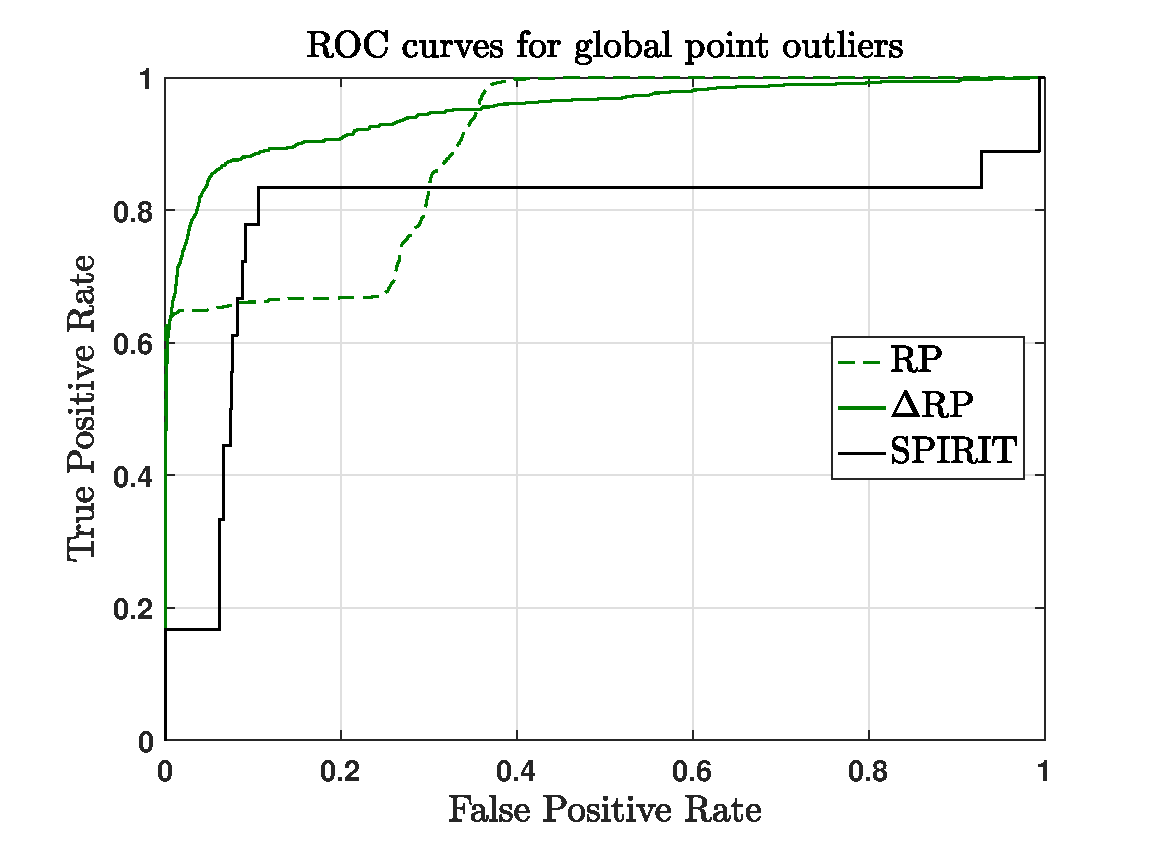
\includegraphics[scale=0.28]{analysis/ROCs_point}
	\end{minipage}
	\begin{minipage}{0.333\textwidth}
		\centering
		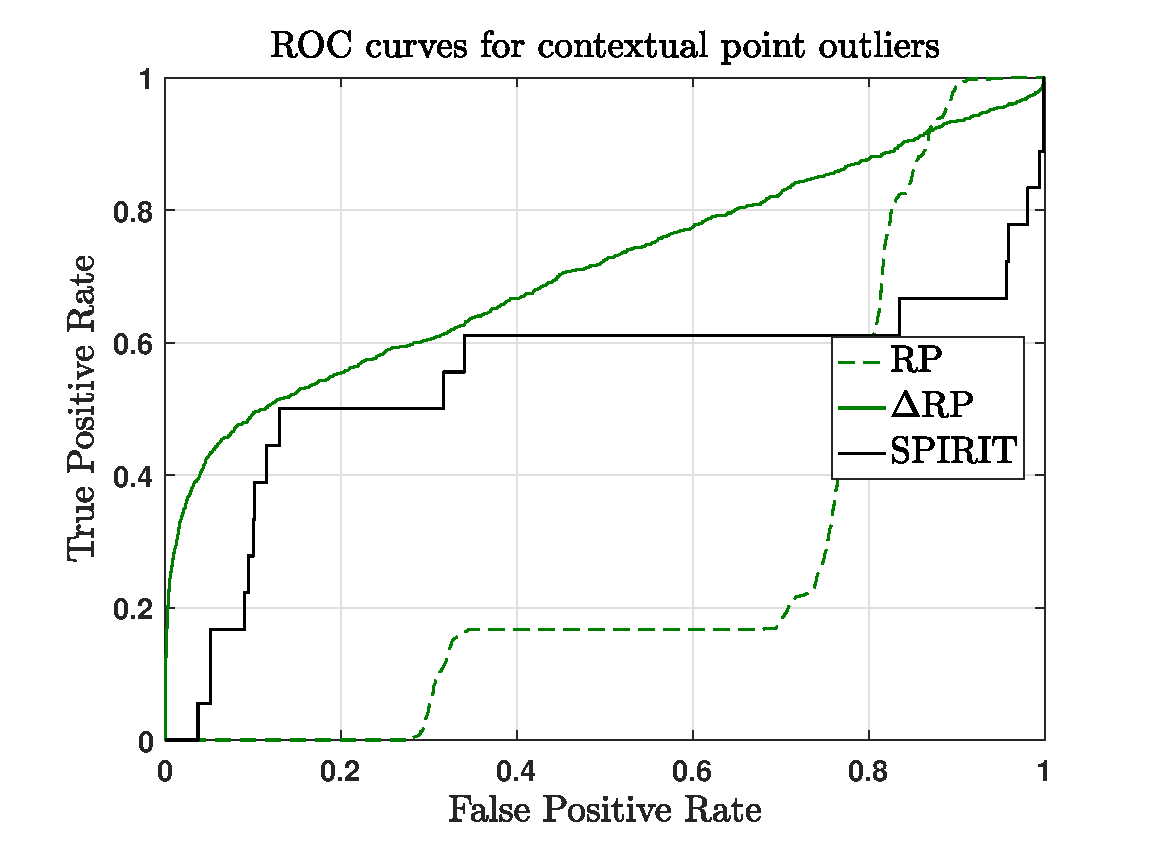
\includegraphics[scale=0.28]{analysis/ROCs_contextual}
	\end{minipage}
	\begin{minipage}{0.333\textwidth}
		\centering
		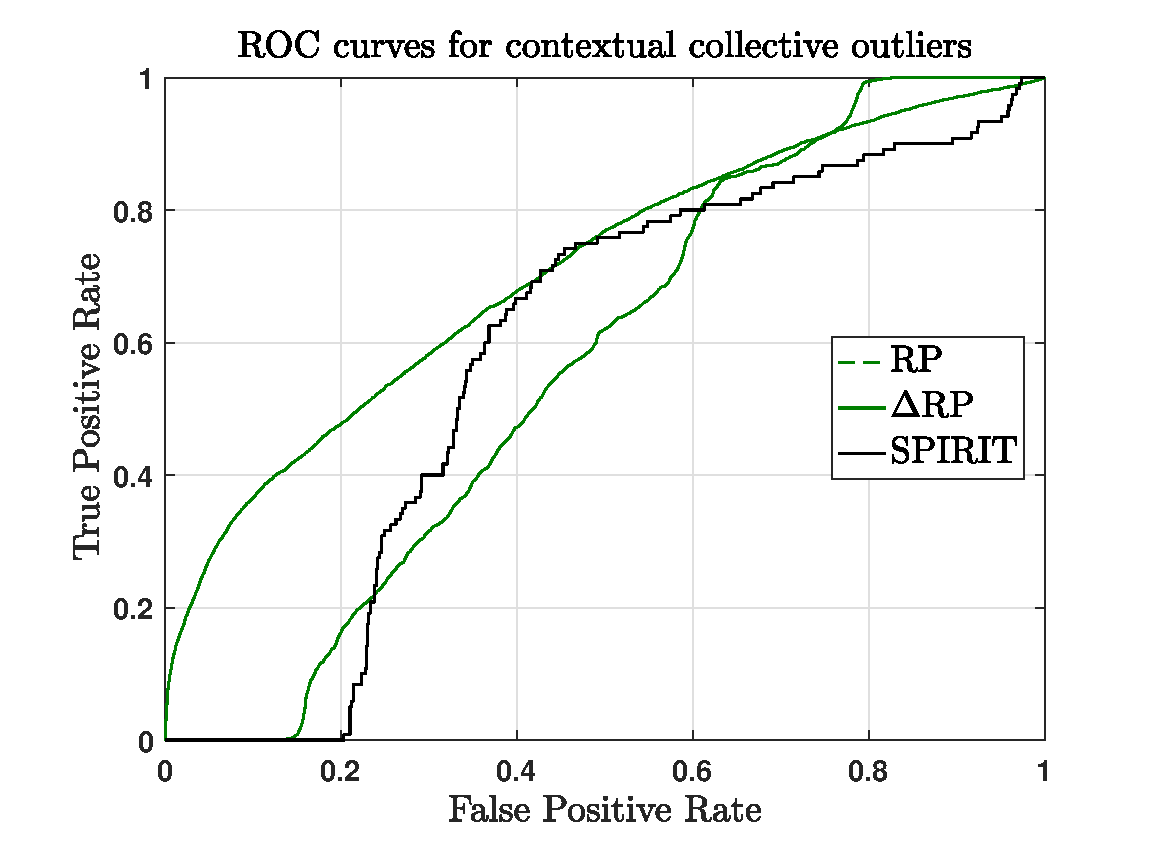
\includegraphics[scale=0.28]{analysis/ROCs_collective}
	\end{minipage}
	\caption{ROC curves of RP, $\Delta$RP and SPIRIT for the three general outlier types.}
	\label{fig:analysis_rocs_point}
\end{figure}


\section{Conclusions}
\label{sec:analysis_concluding}
In this chapter we started with an analysis of the RP method and its performance in the context of unsupervised online outlier detection in multivariate time series. To provide a more thorough understanding of the method, we first showed what actually happens under the hood of the RP method. After gaining these insights we focused, in particular, on the performance in the light of the challenges imposed by our problem context as summarized in table \ref{tab:analysis_evaluation}. To that end, we started with a bird's-eye view of the RP method in comparison to the baseline SPIRIT to determine the effects of the number of projection vectors $k$. As the RP method has difficulties with finding contextual outliers, we adopted a slightly different interpretation (referred to as $\Delta$RP) of the outlier scores which is explained in section \ref{sec:analysis_contextual}. The effectiveness of $\Delta$RP for finding contextual outliers has been evaluated accordingly. Finally, we analysed the performance of the methods when deployed in online mode with fixed parameter settings.

In table \ref{tab:analysis_qualcomp} we provide a qualitative comparison given the evaluation criteria as presented in \ref{tab:intro_characteristics} based on the observations we made in this analysis. We assigned a `$+$' (plus) in case a method was evaluated as best compared to its opponents given a criterion. A `$-$' (minus) is assigned if its performance was not as good as the best method, or a `$/$' (slash) in case the experiments with real-world data are considered necessary to come to a conclusion.

\begin{table}[h]
	\centering
	\vspace{-0.05cm}
	\caption{Evaluation based on the analysis.}
	\label{tab:analysis_qualcomp}
	\begin{tabular}{l c c c}
		\toprule
		\textbf{Evaluation criterion} 		& \textbf{RP} 	& \textbf{$\Delta$RP} & \textbf{SPIRIT} \\ \midrule
		Time needed to process data points 	&  		$+$		&  		$-$		& $-$ \\[0.1cm]
		Dependence on history of stream 	& 		$+$		& 		$+$		& $-$ \\[0.1cm]
		Amount of prior information needed 	& 		$+$		& 		$-$		& $-$ \\[0.1cm]
		Sensitivity of detection performance to parameters 		&	$+$	& 	$-$ 	& $-$ \\
		\midrule
		Generalizability of performances to	different data sets & $/$ & $/$	& $/$ \\[0.1cm]
		Generalizability of performances to different outlier types & $-$	& $+$	& $-$\\
		\midrule
		Influence of $d$ and $n$ on detection performance 		& $/$ & $/$ & $/$ \\[0.1cm]
		Influence of $d$ on runtime	performance	& $+$ & $+$ & $-$ \\
		\bottomrule		
	\end{tabular}
\vspace{-0.1cm}
\end{table}

Starting with the runtime performance, the RP method logically appeared to be significantly faster than $\Delta$RP and SPIRIT. This is mainly because $\Delta$RP runs the RP method $2m$ times, making the default RP method always be the better choice with regard to runtime performance. SPIRIT would be a good choice in case the time series are strongly correlated such that only a few principal coefficient vectors have to be estimated.

Considering the amount of history consumed by a method, adding a sliding window makes SPIRIT its detection performance less sensitive to its parameters. The RP-based methods only benefit a little from a window for contextual outliers. SPIRIT incorporates an additional parameter, forgetting factor $\lambda$, which influences the adaptiveness of the principal coefficient vectors towards the more recent or early history of the data stream. The RP method does not exploit temporal relations by default.

The performance of SPIRIT also relies on the estimated explained variance bounds $f_{\hat{E}}$ (lower) and $F_{\hat{E}}$ (upper), making the number of parameters $2$ in total. Throughout the analysis it turned out that the detection and runtime performances are both sensitive to particularly the variance bounds. This sensitivity also made SPIRIT perform not as good as $\Delta$RP when we analysed the detection performances under fixed parameters in online mode. The default RP method seemed to be parameter-free as it performs best with a single projection vector ($k=1$) for the different outlier types. Increasing the number of projection vectors $k$ for the default RP method only decreases the detection performance a little. $\Delta$RP relies on $1$ parameter, the number of predictors $m$ used to derive an outlier score. Its performance increases smoothly proportionally to the number of predictors $m$ used. The influence of $m$ on the AUC is higher than $k$ for the RP method.

The evaluation regarding the generalizability of the performances of the methods to differently structured data sets is left open as the analysis was conducted with just one data set. We did observe that the detection performance of the methods are sensitive to the mean and range of the data (see appendix \ref{app:analysis}). However, we are also interested in the stability of the performance given different data sets. This is assessed in chapter \ref{chap:experiments}.

We did get a sufficient impression of the generalizability of the methods with respect to the different types of outliers. From the bird's-eye view of the detection performance it became clear that SPIRIT has potential to yield a good AUC for all outlier types. Yet its detection performance suffers from its sensitivity to the parameters. If the analyst has a reasonable understanding of the proper values for the variance bounds to capture the principal behaviour of the time series, SPIRIT might outperform the proposed methods. If the analyst cannot rely on such assumptions, $\Delta$RP will be the better choice, where the default RP method only detects global point outliers well.

Finally, we are also interested in the scalability of the RP-based methods towards high-dimensional data sets. So far, the detection performance of the methods seemed relatively insensitive to the dimensionality of the data. The experiments in chapter \ref{chap:experiments} with differently sized data sets should point out whether the dimensionality has significant impact on the detection performance. When it comes to the runtime performance, we know by the analytical runtime bounds already that the RP-based methods scale better to high $d$ than SPIRIT. That is, the runtime of SPIRIT depends quadratically on $k$ which for SPIRIT is only low if the time series are sufficiently correlated.

